% Options for packages loaded elsewhere
\PassOptionsToPackage{unicode}{hyperref}
\PassOptionsToPackage{hyphens}{url}
%
\documentclass[
]{article}
\usepackage{amsmath,amssymb}
\usepackage{lmodern}
\usepackage{iftex}
\ifPDFTeX
  \usepackage[T1]{fontenc}
  \usepackage[utf8]{inputenc}
  \usepackage{textcomp} % provide euro and other symbols
\else % if luatex or xetex
  \usepackage{unicode-math}
  \defaultfontfeatures{Scale=MatchLowercase}
  \defaultfontfeatures[\rmfamily]{Ligatures=TeX,Scale=1}
\fi
% Use upquote if available, for straight quotes in verbatim environments
\IfFileExists{upquote.sty}{\usepackage{upquote}}{}
\IfFileExists{microtype.sty}{% use microtype if available
  \usepackage[]{microtype}
  \UseMicrotypeSet[protrusion]{basicmath} % disable protrusion for tt fonts
}{}
\makeatletter
\@ifundefined{KOMAClassName}{% if non-KOMA class
  \IfFileExists{parskip.sty}{%
    \usepackage{parskip}
  }{% else
    \setlength{\parindent}{0pt}
    \setlength{\parskip}{6pt plus 2pt minus 1pt}}
}{% if KOMA class
  \KOMAoptions{parskip=half}}
\makeatother
\usepackage{xcolor}
\usepackage[margin=1in]{geometry}
\usepackage{color}
\usepackage{fancyvrb}
\newcommand{\VerbBar}{|}
\newcommand{\VERB}{\Verb[commandchars=\\\{\}]}
\DefineVerbatimEnvironment{Highlighting}{Verbatim}{commandchars=\\\{\}}
% Add ',fontsize=\small' for more characters per line
\usepackage{framed}
\definecolor{shadecolor}{RGB}{248,248,248}
\newenvironment{Shaded}{\begin{snugshade}}{\end{snugshade}}
\newcommand{\AlertTok}[1]{\textcolor[rgb]{0.94,0.16,0.16}{#1}}
\newcommand{\AnnotationTok}[1]{\textcolor[rgb]{0.56,0.35,0.01}{\textbf{\textit{#1}}}}
\newcommand{\AttributeTok}[1]{\textcolor[rgb]{0.77,0.63,0.00}{#1}}
\newcommand{\BaseNTok}[1]{\textcolor[rgb]{0.00,0.00,0.81}{#1}}
\newcommand{\BuiltInTok}[1]{#1}
\newcommand{\CharTok}[1]{\textcolor[rgb]{0.31,0.60,0.02}{#1}}
\newcommand{\CommentTok}[1]{\textcolor[rgb]{0.56,0.35,0.01}{\textit{#1}}}
\newcommand{\CommentVarTok}[1]{\textcolor[rgb]{0.56,0.35,0.01}{\textbf{\textit{#1}}}}
\newcommand{\ConstantTok}[1]{\textcolor[rgb]{0.00,0.00,0.00}{#1}}
\newcommand{\ControlFlowTok}[1]{\textcolor[rgb]{0.13,0.29,0.53}{\textbf{#1}}}
\newcommand{\DataTypeTok}[1]{\textcolor[rgb]{0.13,0.29,0.53}{#1}}
\newcommand{\DecValTok}[1]{\textcolor[rgb]{0.00,0.00,0.81}{#1}}
\newcommand{\DocumentationTok}[1]{\textcolor[rgb]{0.56,0.35,0.01}{\textbf{\textit{#1}}}}
\newcommand{\ErrorTok}[1]{\textcolor[rgb]{0.64,0.00,0.00}{\textbf{#1}}}
\newcommand{\ExtensionTok}[1]{#1}
\newcommand{\FloatTok}[1]{\textcolor[rgb]{0.00,0.00,0.81}{#1}}
\newcommand{\FunctionTok}[1]{\textcolor[rgb]{0.00,0.00,0.00}{#1}}
\newcommand{\ImportTok}[1]{#1}
\newcommand{\InformationTok}[1]{\textcolor[rgb]{0.56,0.35,0.01}{\textbf{\textit{#1}}}}
\newcommand{\KeywordTok}[1]{\textcolor[rgb]{0.13,0.29,0.53}{\textbf{#1}}}
\newcommand{\NormalTok}[1]{#1}
\newcommand{\OperatorTok}[1]{\textcolor[rgb]{0.81,0.36,0.00}{\textbf{#1}}}
\newcommand{\OtherTok}[1]{\textcolor[rgb]{0.56,0.35,0.01}{#1}}
\newcommand{\PreprocessorTok}[1]{\textcolor[rgb]{0.56,0.35,0.01}{\textit{#1}}}
\newcommand{\RegionMarkerTok}[1]{#1}
\newcommand{\SpecialCharTok}[1]{\textcolor[rgb]{0.00,0.00,0.00}{#1}}
\newcommand{\SpecialStringTok}[1]{\textcolor[rgb]{0.31,0.60,0.02}{#1}}
\newcommand{\StringTok}[1]{\textcolor[rgb]{0.31,0.60,0.02}{#1}}
\newcommand{\VariableTok}[1]{\textcolor[rgb]{0.00,0.00,0.00}{#1}}
\newcommand{\VerbatimStringTok}[1]{\textcolor[rgb]{0.31,0.60,0.02}{#1}}
\newcommand{\WarningTok}[1]{\textcolor[rgb]{0.56,0.35,0.01}{\textbf{\textit{#1}}}}
\usepackage{longtable,booktabs,array}
\usepackage{calc} % for calculating minipage widths
% Correct order of tables after \paragraph or \subparagraph
\usepackage{etoolbox}
\makeatletter
\patchcmd\longtable{\par}{\if@noskipsec\mbox{}\fi\par}{}{}
\makeatother
% Allow footnotes in longtable head/foot
\IfFileExists{footnotehyper.sty}{\usepackage{footnotehyper}}{\usepackage{footnote}}
\makesavenoteenv{longtable}
\usepackage{graphicx}
\makeatletter
\def\maxwidth{\ifdim\Gin@nat@width>\linewidth\linewidth\else\Gin@nat@width\fi}
\def\maxheight{\ifdim\Gin@nat@height>\textheight\textheight\else\Gin@nat@height\fi}
\makeatother
% Scale images if necessary, so that they will not overflow the page
% margins by default, and it is still possible to overwrite the defaults
% using explicit options in \includegraphics[width, height, ...]{}
\setkeys{Gin}{width=\maxwidth,height=\maxheight,keepaspectratio}
% Set default figure placement to htbp
\makeatletter
\def\fps@figure{htbp}
\makeatother
\setlength{\emergencystretch}{3em} % prevent overfull lines
\providecommand{\tightlist}{%
  \setlength{\itemsep}{0pt}\setlength{\parskip}{0pt}}
\setcounter{secnumdepth}{-\maxdimen} % remove section numbering
\ifLuaTeX
  \usepackage{selnolig}  % disable illegal ligatures
\fi
\IfFileExists{bookmark.sty}{\usepackage{bookmark}}{\usepackage{hyperref}}
\IfFileExists{xurl.sty}{\usepackage{xurl}}{} % add URL line breaks if available
\urlstyle{same} % disable monospaced font for URLs
\hypersetup{
  pdftitle={glurs},
  pdfauthor={Alexander Bates},
  hidelinks,
  pdfcreator={LaTeX via pandoc}}

\title{glurs}
\author{Alexander Bates}
\date{2023-11-03}

\begin{document}
\maketitle

\begin{Shaded}
\begin{Highlighting}[]
\FunctionTok{library}\NormalTok{(ggplot2)}
\FunctionTok{library}\NormalTok{(Matrix)}
\FunctionTok{library}\NormalTok{(cowplot)}
\FunctionTok{library}\NormalTok{(Seurat)}
\end{Highlighting}
\end{Shaded}

\begin{verbatim}
## Attaching SeuratObject
\end{verbatim}

\begin{verbatim}
## Seurat v4 was just loaded with SeuratObject v5; disabling v5 assays and
## validation routines, and ensuring assays work in strict v3/v4
## compatibility mode
\end{verbatim}

\begin{Shaded}
\begin{Highlighting}[]
\FunctionTok{library}\NormalTok{(tidyverse)}
\end{Highlighting}
\end{Shaded}

\begin{verbatim}
## -- Attaching packages --------------------------------------- tidyverse 1.3.2
## --
\end{verbatim}

\begin{verbatim}
## v tibble  3.2.1     v dplyr   1.1.3
## v tidyr   1.3.0     v stringr 1.5.0
## v readr   2.1.4     v forcats 0.5.2
## v purrr   1.0.2     
## -- Conflicts ------------------------------------------ tidyverse_conflicts() --
## x tidyr::expand() masks Matrix::expand()
## x dplyr::filter() masks stats::filter()
## x dplyr::lag()    masks stats::lag()
## x tidyr::pack()   masks Matrix::pack()
## x tidyr::unpack() masks Matrix::unpack()
\end{verbatim}

\begin{Shaded}
\begin{Highlighting}[]
\FunctionTok{library}\NormalTok{(plyr)}
\end{Highlighting}
\end{Shaded}

\begin{verbatim}
## ------------------------------------------------------------------------------
## You have loaded plyr after dplyr - this is likely to cause problems.
## If you need functions from both plyr and dplyr, please load plyr first, then dplyr:
## library(plyr); library(dplyr)
## ------------------------------------------------------------------------------
## 
## Attaching package: 'plyr'
## 
## The following objects are masked from 'package:dplyr':
## 
##     arrange, count, desc, failwith, id, mutate, rename, summarise,
##     summarize
## 
## The following object is masked from 'package:purrr':
## 
##     compact
\end{verbatim}

\begin{Shaded}
\begin{Highlighting}[]
\FunctionTok{library}\NormalTok{(SingleCellExperiment)}
\end{Highlighting}
\end{Shaded}

\begin{verbatim}
## Loading required package: SummarizedExperiment
## Loading required package: MatrixGenerics
## Loading required package: matrixStats
## 
## Attaching package: 'matrixStats'
## 
## The following object is masked from 'package:plyr':
## 
##     count
## 
## The following object is masked from 'package:dplyr':
## 
##     count
## 
## 
## Attaching package: 'MatrixGenerics'
## 
## The following objects are masked from 'package:matrixStats':
## 
##     colAlls, colAnyNAs, colAnys, colAvgsPerRowSet, colCollapse,
##     colCounts, colCummaxs, colCummins, colCumprods, colCumsums,
##     colDiffs, colIQRDiffs, colIQRs, colLogSumExps, colMadDiffs,
##     colMads, colMaxs, colMeans2, colMedians, colMins, colOrderStats,
##     colProds, colQuantiles, colRanges, colRanks, colSdDiffs, colSds,
##     colSums2, colTabulates, colVarDiffs, colVars, colWeightedMads,
##     colWeightedMeans, colWeightedMedians, colWeightedSds,
##     colWeightedVars, rowAlls, rowAnyNAs, rowAnys, rowAvgsPerColSet,
##     rowCollapse, rowCounts, rowCummaxs, rowCummins, rowCumprods,
##     rowCumsums, rowDiffs, rowIQRDiffs, rowIQRs, rowLogSumExps,
##     rowMadDiffs, rowMads, rowMaxs, rowMeans2, rowMedians, rowMins,
##     rowOrderStats, rowProds, rowQuantiles, rowRanges, rowRanks,
##     rowSdDiffs, rowSds, rowSums2, rowTabulates, rowVarDiffs, rowVars,
##     rowWeightedMads, rowWeightedMeans, rowWeightedMedians,
##     rowWeightedSds, rowWeightedVars
## 
## Loading required package: GenomicRanges
## Loading required package: stats4
## Loading required package: BiocGenerics
## 
## Attaching package: 'BiocGenerics'
## 
## The following objects are masked from 'package:dplyr':
## 
##     combine, intersect, setdiff, union
## 
## The following object is masked from 'package:SeuratObject':
## 
##     intersect
## 
## The following objects are masked from 'package:stats':
## 
##     IQR, mad, sd, var, xtabs
## 
## The following objects are masked from 'package:base':
## 
##     anyDuplicated, append, as.data.frame, basename, cbind, colnames,
##     dirname, do.call, duplicated, eval, evalq, Filter, Find, get, grep,
##     grepl, intersect, is.unsorted, lapply, Map, mapply, match, mget,
##     order, paste, pmax, pmax.int, pmin, pmin.int, Position, rank,
##     rbind, Reduce, rownames, sapply, setdiff, sort, table, tapply,
##     union, unique, unsplit, which.max, which.min
## 
## Loading required package: S4Vectors
## 
## Attaching package: 'S4Vectors'
## 
## The following object is masked from 'package:plyr':
## 
##     rename
## 
## The following objects are masked from 'package:dplyr':
## 
##     first, rename
## 
## The following object is masked from 'package:tidyr':
## 
##     expand
## 
## The following objects are masked from 'package:Matrix':
## 
##     expand, unname
## 
## The following objects are masked from 'package:base':
## 
##     expand.grid, I, unname
## 
## Loading required package: IRanges
## 
## Attaching package: 'IRanges'
## 
## The following object is masked from 'package:plyr':
## 
##     desc
## 
## The following objects are masked from 'package:dplyr':
## 
##     collapse, desc, slice
## 
## The following object is masked from 'package:purrr':
## 
##     reduce
## 
## Loading required package: GenomeInfoDb
## Loading required package: Biobase
## Welcome to Bioconductor
## 
##     Vignettes contain introductory material; view with
##     'browseVignettes()'. To cite Bioconductor, see
##     'citation("Biobase")', and for packages 'citation("pkgname")'.
## 
## 
## Attaching package: 'Biobase'
## 
## The following object is masked from 'package:MatrixGenerics':
## 
##     rowMedians
## 
## The following objects are masked from 'package:matrixStats':
## 
##     anyMissing, rowMedians
## 
## 
## Attaching package: 'SummarizedExperiment'
## 
## The following object is masked from 'package:SeuratObject':
## 
##     Assays
## 
## The following object is masked from 'package:Seurat':
## 
##     Assays
\end{verbatim}

\begin{Shaded}
\begin{Highlighting}[]
\FunctionTok{library}\NormalTok{(matrixStats)}
\FunctionTok{library}\NormalTok{(umap)}
\FunctionTok{library}\NormalTok{(foreach)}
\end{Highlighting}
\end{Shaded}

\begin{verbatim}
## 
## Attaching package: 'foreach'
## 
## The following objects are masked from 'package:purrr':
## 
##     accumulate, when
\end{verbatim}

\begin{Shaded}
\begin{Highlighting}[]
\FunctionTok{library}\NormalTok{(DoubletFinder)}

\CommentTok{\# Load the data we need}
\FunctionTok{load}\NormalTok{(}\StringTok{"\textasciitilde{}/projects/wilson{-}lab/nat{-}tech/data/park\_et\_al\_2022/GSE207799\_Thirst2\_SCT\_trimPlus.Robj"}\NormalTok{)}
\NormalTok{Thirst2\_SCT\_trimPlus }\OtherTok{\textless{}{-}} \FunctionTok{UpdateSeuratObject}\NormalTok{(}\AttributeTok{object =}\NormalTok{ Thirst2\_SCT\_trimPlus)}
\end{Highlighting}
\end{Shaded}

\begin{verbatim}
## Validating object structure
## Updating object slots
## Ensuring keys are in the proper structure
## Updating matrix keys for DimReduc 'pca'
## Updating matrix keys for DimReduc 'umap'
## Ensuring keys are in the proper structure
## Ensuring feature names don't have underscores or pipes
## Updating slots in RNA
## Updating slots in SCT
## Updating slots in integrated
## Updating slots in integrated_nn
## Setting default assay of integrated_nn to integrated
## Updating slots in integrated_snn
## Setting default assay of integrated_snn to integrated
## Updating slots in pca
## Updating slots in umap
## Setting umap DimReduc to global
## No assay information could be found for FindIntegrationAnchors
\end{verbatim}

\begin{verbatim}
## Warning: Adding a command log without an assay associated with it
\end{verbatim}

\begin{verbatim}
## No assay information could be found for PairwiseIntegrateReference
\end{verbatim}

\begin{verbatim}
## Warning: Adding a command log without an assay associated with it
\end{verbatim}

\begin{verbatim}
## Setting assay used for JackStraw.integrated.pca to integrated
## No assay information could be found for ScoreJackStraw
\end{verbatim}

\begin{verbatim}
## Warning: Adding a command log without an assay associated with it
\end{verbatim}

\begin{verbatim}
## Setting assay used for RunPCA.integrated to integrated
## Setting assay used for FindNeighbors.integrated.pca to integrated
## No assay information could be found for FindClusters
\end{verbatim}

\begin{verbatim}
## Warning: Adding a command log without an assay associated with it
\end{verbatim}

\begin{verbatim}
## Setting assay used for RunUMAP.integrated.pca to integrated
## Validating object structure for Assay 'RNA'
## Validating object structure for Assay 'SCT'
## Validating object structure for Assay 'integrated'
## Validating object structure for Graph 'integrated_nn'
## Validating object structure for Graph 'integrated_snn'
## Validating object structure for DimReduc 'pca'
## Validating object structure for DimReduc 'umap'
## Object representation is consistent with the most current Seurat version
\end{verbatim}

\begin{Shaded}
\begin{Highlighting}[]
\FunctionTok{DefaultAssay}\NormalTok{(Thirst2\_SCT\_trimPlus) }\OtherTok{\textless{}{-}} \StringTok{"SCT"}
\FunctionTok{load}\NormalTok{(}\StringTok{"\textasciitilde{}/projects/wilson{-}lab/nat{-}tech/data/park\_et\_al\_2022/GSE207799\_Thirst2\_celltypes.Robj"}\NormalTok{)}
\CommentTok{\#Thirst2\_celltypes \textless{}{-} UpdateSeuratObject(object = Thirst2\_celltypes)}
\CommentTok{\#DefaultAssay(Thirst2\_celltypes) \textless{}{-} "SCT"}

\CommentTok{\# knit options}
\CommentTok{\#dir.create(\textquotesingle{}images/GluR\_scRNA\textquotesingle{}, recursive = TRUE, showWarnings = FALSE)}
\NormalTok{knitr}\SpecialCharTok{::}\NormalTok{opts\_chunk}\SpecialCharTok{$}\FunctionTok{set}\NormalTok{(}\AttributeTok{echo =} \ConstantTok{FALSE}\NormalTok{,}
                      \AttributeTok{include =} \ConstantTok{TRUE}\NormalTok{,}
                      \AttributeTok{message =} \ConstantTok{FALSE}\NormalTok{,}
                      \AttributeTok{warning =} \ConstantTok{FALSE}\NormalTok{,}
                      \AttributeTok{fig.path=}\StringTok{\textquotesingle{}\textasciitilde{}/projects/wilson{-}lab/nat{-}tech/images/GluR\_scRNA/\textquotesingle{}}\NormalTok{,}
                      \AttributeTok{dev =} \FunctionTok{c}\NormalTok{(}\StringTok{\textquotesingle{}pdf\textquotesingle{}}\NormalTok{, }\StringTok{\textquotesingle{}png\textquotesingle{}}\NormalTok{),}
                      \AttributeTok{fig\_caption =} \ConstantTok{TRUE}\NormalTok{,}
                      \AttributeTok{fig.align =} \StringTok{\textquotesingle{}center\textquotesingle{}}\NormalTok{,}
                      \AttributeTok{fig.height =} \DecValTok{6}\NormalTok{,}
                      \AttributeTok{fig.width =} \DecValTok{8}\NormalTok{,}
                      \FunctionTok{pdf.options}\NormalTok{(}\AttributeTok{encoding =} \StringTok{"ISOLatin9.enc"}\NormalTok{),}
                      \AttributeTok{rgl=}\ConstantTok{TRUE}\NormalTok{)}
\end{Highlighting}
\end{Shaded}

\begin{longtable}[]{@{}
  >{\raggedleft\arraybackslash}p{(\columnwidth - 12\tabcolsep) * \real{0.1370}}
  >{\raggedleft\arraybackslash}p{(\columnwidth - 12\tabcolsep) * \real{0.1507}}
  >{\raggedleft\arraybackslash}p{(\columnwidth - 12\tabcolsep) * \real{0.0822}}
  >{\raggedleft\arraybackslash}p{(\columnwidth - 12\tabcolsep) * \real{0.0822}}
  >{\raggedleft\arraybackslash}p{(\columnwidth - 12\tabcolsep) * \real{0.1370}}
  >{\raggedright\arraybackslash}p{(\columnwidth - 12\tabcolsep) * \real{0.2603}}
  >{\raggedright\arraybackslash}p{(\columnwidth - 12\tabcolsep) * \real{0.1507}}@{}}
\toprule()
\begin{minipage}[b]{\linewidth}\raggedleft
p\_val
\end{minipage} & \begin{minipage}[b]{\linewidth}\raggedleft
avg\_log2FC
\end{minipage} & \begin{minipage}[b]{\linewidth}\raggedleft
pct.1
\end{minipage} & \begin{minipage}[b]{\linewidth}\raggedleft
pct.2
\end{minipage} & \begin{minipage}[b]{\linewidth}\raggedleft
p\_val\_adj
\end{minipage} & \begin{minipage}[b]{\linewidth}\raggedright
cluster
\end{minipage} & \begin{minipage}[b]{\linewidth}\raggedright
gene
\end{minipage} \\
\midrule()
\endhead
0.0000000 & -1.1506983 & 0.016 & 0.884 & 0.0000000 & 17\_SurfaceGlia &
GluClalpha \\
0.0000000 & -1.0449139 & 0.111 & 0.884 & 0.0000000 & 25\_dFB/vFB &
GluClalpha \\
0.0000000 & 1.0093487 & 1.000 & 0.523 & 0.0000000 & 36\_Glut & GluRIA \\
0.0000000 & -0.9847574 & 0.161 & 0.886 & 0.0000000 & 13\_LF-EB &
GluClalpha \\
0.0000000 & -0.9617073 & 0.133 & 0.883 & 0.0000000 & 18\_SurfaceGlia &
GluClalpha \\
0.0000000 & -0.9504382 & 0.159 & 0.925 & 0.0000000 & 17\_SurfaceGlia &
CG11155 \\
0.0000000 & -0.8586078 & 0.233 & 0.924 & 0.0000000 & 18\_SurfaceGlia &
CG11155 \\
0.0000000 & -0.8528569 & 0.267 & 0.883 & 0.0000000 & 41\_mFB &
GluClalpha \\
0.0000000 & 0.8193333 & 0.962 & 0.543 & 0.0000000 & 36\_Glut & GluRIB \\
0.0000000 & -0.7605077 & 0.377 & 0.884 & 0.0000000 & 33\_GABA &
GluClalpha \\
0.0000000 & 0.7582331 & 1.000 & 0.375 & 0.0000000 & 14\_DA-PAM &
Nmdar2 \\
0.0000000 & -0.7405913 & 0.412 & 0.890 & 0.0000000 & 1\_primeKCs &
GluClalpha \\
0.0000000 & 0.7239828 & 0.917 & 0.375 & 0.0000000 & 21\_DA-PAM &
Nmdar2 \\
0.0000000 & -0.7221806 & 0.436 & 0.884 & 0.0000000 & 13\_CortexGlia &
GluClalpha \\
0.0000000 & 0.7069787 & 0.917 & 0.375 & 0.0000000 & 23\_DA & Nmdar2 \\
0.0000000 & 0.7039871 & 0.894 & 0.375 & 0.0000000 & 2\_DA-PAM &
Nmdar2 \\
0.0000000 & 0.6990014 & 0.988 & 0.883 & 0.0000000 & 49\_ACh &
GluClalpha \\
0.0000000 & -0.6867421 & 0.389 & 0.884 & 0.0000000 & 51\_ACh &
GluClalpha \\
0.0000000 & -0.6864850 & 0.451 & 0.883 & 0.0000000 & 15\_primeKCs &
GluClalpha \\
0.0000000 & -0.6780229 & 0.000 & 0.544 & 0.0000000 & 1\_DA-PAM &
GluRIB \\
0.0000000 & -0.6778610 & 0.000 & 0.544 & 0.0005465 & 41\_mFB & GluRIB \\
0.0000000 & 0.6713668 & 0.968 & 0.541 & 0.0000000 & 6\_abKCs & GluRIB \\
0.0000000 & -0.6623461 & 0.016 & 0.544 & 0.0000000 & 17\_SurfaceGlia &
GluRIB \\
0.0000000 & -0.6600060 & 0.462 & 0.883 & 0.0001147 & 17\_TA &
GluClalpha \\
0.0000000 & -0.6559261 & 0.022 & 0.544 & 0.0000009 & 3\_DA-PAM &
GluRIB \\
0.0000000 & -0.6494305 & 0.000 & 0.524 & 0.0000000 & 17\_SurfaceGlia &
GluRIA \\
0.0000000 & -0.6492657 & 0.000 & 0.524 & 0.0000025 & 37\_Glut &
GluRIA \\
0.0000000 & -0.6491916 & 0.000 & 0.524 & 0.0001936 & 10\_DA-PAM &
GluRIA \\
0.0000001 & -0.6491586 & 0.000 & 0.524 & 0.0013423 & 41\_mFB & GluRIA \\
0.0000001 & -0.6491586 & 0.000 & 0.524 & 0.0013423 & 14\_DA-PAM &
GluRIA \\
0.0000008 & -0.6491257 & 0.000 & 0.524 & 0.0093779 & 18\_OA & GluRIA \\
0.0000002 & -0.6448970 & 0.033 & 0.544 & 0.0019516 & 14\_DA-PAM &
GluRIB \\
0.0000001 & 0.6431619 & 0.938 & 0.375 & 0.0006525 & 25\_TA & Nmdar2 \\
0.0000013 & -0.6398593 & 0.038 & 0.544 & 0.0153445 & 18\_OA & GluRIB \\
0.0000036 & -0.6367237 & 0.042 & 0.544 & 0.0431921 & 21\_DA-PAM &
GluRIB \\
0.0000000 & -0.6360485 & 0.043 & 0.544 & 0.0000011 & 2\_DA-PAM &
GluRIB \\
0.0000000 & 0.6359503 & 0.951 & 0.522 & 0.0000000 & 8\_primeKCs &
GluRIA \\
0.0000000 & -0.6356722 & 0.014 & 0.524 & 0.0000000 & 51\_ACh & GluRIA \\
0.0000000 & -0.6281674 & 0.021 & 0.524 & 0.0000013 & 2\_DA-PAM &
GluRIA \\
0.0000000 & -0.6276638 & 0.046 & 0.544 & 0.0000000 & 25\_dFB/vFB &
GluRIB \\
0.0000000 & -0.6260372 & 0.019 & 0.524 & 0.0000000 & 25\_dFB/vFB &
GluRIA \\
0.0000000 & -0.6231358 & 0.026 & 0.524 & 0.0001009 & 8\_DA-PAM &
GluRIA \\
0.0000000 & -0.6230886 & 0.596 & 0.885 & 0.0000000 & 4\_EnsheathingGlia
& GluClalpha \\
0.0000001 & -0.6202194 & 0.059 & 0.544 & 0.0008527 & 10\_DA-PAM &
GluRIB \\
0.0000000 & -0.6186720 & 0.058 & 0.545 & 0.0000000 & 41\_ACh & GluRIB \\
0.0000000 & -0.6159374 & 0.030 & 0.525 & 0.0000000 & 13\_LF-EB &
GluRIA \\
0.0000000 & -0.6098092 & 0.070 & 0.544 & 0.0000286 & 37\_Glut &
GluRIB \\
0.0000000 & -0.6082171 & 0.071 & 0.544 & 0.0000475 & 3\_Other-ACh &
GluRIB \\
0.0000000 & -0.6075109 & 0.073 & 0.544 & 0.0000000 & 13\_CortexGlia &
GluRIB \\
0.0000000 & 0.6073442 & 0.921 & 0.532 & 0.0000000 & 2\_abKCs & GluRIB \\
0.0000000 & -0.6065495 & 0.073 & 0.544 & 0.0000789 & 4\_OtherNeurons &
GluRIB \\
0.0000000 & -0.6023873 & 0.048 & 0.524 & 0.0000507 & 3\_Other-ACh &
GluRIA \\
0.0000000 & -0.6010366 & 0.079 & 0.544 & 0.0003625 & 8\_DA-PAM &
GluRIB \\
0.0000000 & -0.6004075 & 0.072 & 0.545 & 0.0000000 & 13\_LF-EB &
GluRIB \\
0.0000000 & -0.5946432 & 0.077 & 0.544 & 0.0000000 & 54\_ACh & GluRIB \\
0.0000000 & -0.5942299 & 0.479 & 0.883 & 0.0000000 & 32\_Glut &
GluClalpha \\
0.0000000 & -0.5899845 & 0.035 & 0.524 & 0.0000000 & 49\_ACh & GluRIA \\
0.0000000 & -0.5894783 & 0.083 & 0.544 & 0.0000000 & 51\_ACh & GluRIB \\
0.0000000 & -0.5874749 & 0.064 & 0.524 & 0.0000000 & 13\_CortexGlia &
GluRIA \\
0.0000000 & -0.5863338 & 0.058 & 0.525 & 0.0000000 & 41\_ACh & GluRIA \\
0.0000000 & 0.5846807 & 0.800 & 0.375 & 0.0000055 & 41\_mFB & Nmdar2 \\
0.0000000 & -0.5830379 & 0.061 & 0.544 & 0.0000000 & 44\_ACh & GluRIB \\
0.0000000 & -0.5827459 & 0.047 & 0.544 & 0.0000000 & 49\_ACh & GluRIB \\
0.0000000 & 0.5810777 & 0.857 & 0.375 & 0.0004522 & 24\_MA\_Other &
Nmdar2 \\
0.0000000 & -0.5797722 & 0.626 & 0.885 & 0.0000000 & 2\_EnsheathingGlia
& GluClalpha \\
0.0000000 & -0.5779113 & 0.061 & 0.524 & 0.0000108 & 1\_DA-PAM &
GluRIA \\
0.0000000 & -0.5719728 & 0.062 & 0.524 & 0.0000000 & 54\_ACh & GluRIA \\
0.0000010 & -0.5705496 & 0.062 & 0.524 & 0.0114590 & 12\_DA-PAM &
GluRIA \\
0.0000254 & -0.5680737 & 0.083 & 0.524 & 0.3030092 & 21\_DA-PAM &
GluRIA \\
0.0000025 & -0.5654423 & 0.067 & 0.524 & 0.0300653 & 18\_SurfaceGlia &
GluRIA \\
0.0000032 & -0.5630186 & 0.100 & 0.544 & 0.0387063 & 18\_SurfaceGlia &
GluRIB \\
0.0000000 & 0.5585035 & 0.846 & 0.375 & 0.0000567 & 17\_TA & Nmdar2 \\
0.0000000 & -0.5583380 & 0.551 & 0.884 & 0.0000000 & 8\_primeKCs &
GluClalpha \\
0.0000002 & -0.5578038 & 0.079 & 0.524 & 0.0020550 & 7\_DA-PAM &
GluRIA \\
0.0000000 & 0.5574679 & 0.940 & 0.543 & 0.0000000 & 0\_TA & GluRIB \\
0.0000000 & 0.5552560 & 0.912 & 0.542 & 0.0000000 & 10\_abKCs &
GluRIB \\
0.0000000 & 0.5521490 & 0.892 & 0.512 & 0.0000000 & 2\_abKCs & GluRIA \\
0.0000000 & -0.5507850 & 0.089 & 0.524 & 0.0002285 & 3\_DA-PAM &
GluRIA \\
0.0000020 & -0.5487284 & 0.094 & 0.544 & 0.0240427 & 12\_DA-PAM &
GluRIB \\
0.0000000 & -0.5473443 & 0.094 & 0.524 & 0.0000000 & 28\_Glut &
GluRIA \\
0.0000000 & 0.5404345 & 0.955 & 0.543 & 0.0000000 & 45\_ACh & GluRIB \\
0.0000000 & -0.5402509 & 0.113 & 0.526 & 0.0000000 & 4\_EnsheathingGlia
& GluRIA \\
0.0000000 & -0.5382324 & 0.117 & 0.528 & 0.0000000 & 1\_Astrocytes &
GluRIA \\
0.0000000 & 0.5374336 & 0.838 & 0.543 & 0.0000000 & 34\_GABA & GluRIB \\
0.0000000 & 0.5360621 & 0.923 & 0.523 & 0.0002882 & 17\_TA & GluRIA \\
0.0000000 & -0.5354654 & 0.150 & 0.544 & 0.0000000 & 50\_ACh & GluRIB \\
0.0000000 & -0.5352200 & 0.123 & 0.546 & 0.0000000 & 29\_ACh & GluRIB \\
0.0000000 & 0.5317588 & 0.903 & 0.522 & 0.0000000 & 6\_abKCs & GluRIA \\
0.0000000 & 0.5264928 & 0.912 & 0.543 & 0.0000000 & 53\_ACh & GluRIB \\
0.0000000 & 0.5254675 & 0.962 & 0.543 & 0.0002250 & 17\_TA & GluRIB \\
0.0000000 & 0.5251801 & 0.928 & 0.523 & 0.0000000 & 45\_ACh & GluRIA \\
0.0000000 & -0.5245584 & 0.102 & 0.526 & 0.0000000 & 29\_ACh & GluRIA \\
0.0000000 & -0.5234928 & 0.586 & 0.884 & 0.0000000 & 9\_abKCs &
GluClalpha \\
0.0000000 & -0.5232046 & 0.161 & 0.548 & 0.0000000 & 1\_Astrocytes &
GluRIB \\
0.0000000 & 0.5231207 & 0.848 & 0.523 & 0.0000000 & 28\_GABA & GluRIA \\
0.0000000 & -0.5215884 & 0.122 & 0.525 & 0.0000000 & 40\_ACh & GluRIA \\
0.0000000 & 0.5211350 & 0.818 & 0.271 & 0.0000000 & 6\_Other-ACh &
Nmdar1 \\
0.0000000 & -0.5170394 & 0.118 & 0.544 & 0.0000000 & 28\_Glut &
GluRIB \\
0.0000000 & -0.5163066 & 0.128 & 0.524 & 0.0000000 & 48\_ACh & GluRIA \\
0.0000000 & -0.5133601 & 0.159 & 0.546 & 0.0000000 & 4\_EnsheathingGlia
& GluRIB \\
0.0000352 & -0.5128830 & 0.143 & 0.524 & 0.4199000 & 16\_DA-PAM &
GluRIA \\
0.0000000 & -0.5107124 & 0.121 & 0.525 & 0.0000000 & 35\_ACh & GluRIA \\
0.0000000 & -0.5103232 & 0.096 & 0.524 & 0.0000000 & 44\_ACh & GluRIA \\
0.0000433 & -0.5094398 & 0.179 & 0.544 & 0.5155618 & 16\_DA-PAM &
GluRIB \\
0.0000000 & 0.4992056 & 0.820 & 0.375 & 0.0000000 & 0\_TA & Nmdar2 \\
0.0000000 & 0.4959187 & 0.855 & 0.522 & 0.0000000 & 10\_abKCs &
GluRIA \\
0.0000000 & -0.4948545 & 0.171 & 0.544 & 0.0000000 & 40\_ACh & GluRIB \\
0.0000000 & -0.4928352 & 0.128 & 0.546 & 0.0000000 & 31\_ACh & GluRIB \\
0.0000054 & -0.4914255 & 0.139 & 0.524 & 0.0642284 & 5\_Other-ACh &
GluRIA \\
0.0000000 & -0.4878463 & 0.119 & 0.526 & 0.0000000 & 31\_ACh & GluRIA \\
0.0000000 & -0.4848409 & 0.765 & 0.884 & 0.0000000 & 5\_EnsheathingGlia
& GluClalpha \\
0.0000000 & -0.4817554 & 0.208 & 0.546 & 0.0000000 & 2\_EnsheathingGlia
& GluRIB \\
0.0000000 & -0.4815291 & 0.610 & 0.883 & 0.0000727 & 4\_OtherNeurons &
GluClalpha \\
0.0000000 & 0.4787491 & 1.000 & 0.883 & 0.0000000 & 36\_GABA &
GluClalpha \\
0.0064745 & -0.4779047 & 0.214 & 0.543 & 1.0000000 & 11\_OtherNeurons &
GluRIB \\
0.0000000 & -0.4756607 & 0.180 & 0.526 & 0.0000000 & 2\_EnsheathingGlia
& GluRIA \\
0.0000000 & 0.4699396 & 0.950 & 0.883 & 0.0000000 & 27\_GABA &
GluClalpha \\
0.0000000 & -0.4697542 & 0.165 & 0.544 & 0.0000000 & 29\_GABA &
GluRIB \\
0.0000000 & -0.4696971 & 0.181 & 0.545 & 0.0000000 & 37\_ACh & GluRIB \\
0.0000000 & -0.4670245 & 0.176 & 0.545 & 0.0000000 & 35\_ACh & GluRIB \\
0.0000000 & -0.4668864 & 0.190 & 0.525 & 0.0000000 & 5\_EnsheathingGlia
& GluRIA \\
0.0000049 & -0.4661611 & 0.195 & 0.524 & 0.0585100 & 4\_OtherNeurons &
GluRIA \\
0.0000000 & -0.4648074 & 0.175 & 0.524 & 0.0000019 & 50\_ACh & GluRIA \\
0.0000000 & -0.4628657 & 0.230 & 0.545 & 0.0000000 & 5\_EnsheathingGlia
& GluRIB \\
0.0000219 & -0.4590655 & 0.118 & 0.524 & 0.2607507 & 11\_DA-PAM &
GluRIA \\
0.0005554 & -0.4577006 & 0.526 & 0.883 & 1.0000000 & 10\_ClockNeurons &
GluClalpha \\
0.0000437 & -0.4517282 & 0.206 & 0.544 & 0.5210516 & 11\_DA-PAM &
GluRIB \\
0.0000000 & 0.4508400 & 0.724 & 0.271 & 0.0000000 & 47\_ACh & Nmdar1 \\
0.0025888 & -0.4498794 & 0.571 & 0.883 & 1.0000000 & 11\_OtherNeurons &
GluClalpha \\
0.0000234 & -0.4494748 & 0.167 & 0.544 & 0.2793314 & 5\_Other-ACh &
GluRIB \\
0.0000000 & 0.4476959 & 0.935 & 0.542 & 0.0000000 & 8\_primeKCs &
GluRIB \\
0.0000000 & 0.4471555 & 0.986 & 0.883 & 0.0000000 & 35\_GABA &
GluClalpha \\
0.0000000 & -0.4454420 & 0.158 & 0.525 & 0.0000000 & 39\_ACh & GluRIA \\
0.0006207 & -0.4427835 & 0.167 & 0.524 & 1.0000000 & 22\_MA\_Other &
GluRIA \\
0.0000008 & -0.4420494 & 0.192 & 0.524 & 0.0095044 & 2\_IPCs & GluRIA \\
0.0000000 & -0.4407654 & 0.769 & 0.883 & 0.0000002 & 2\_IPCs &
GluClalpha \\
0.0002041 & 0.4385865 & 0.833 & 0.523 & 1.0000000 & 23\_DA & GluRIA \\
0.0000000 & 0.4380699 & 0.900 & 0.523 & 0.0000014 & 0\_TA & GluRIA \\
0.0000446 & 0.4319590 & 0.833 & 0.543 & 0.5316917 & 20\_DA-PAM &
GluRIB \\
0.0001423 & -0.4256509 & 0.129 & 0.524 & 1.0000000 & 7\_Other-ACh &
GluRIA \\
0.0000000 & -0.4250177 & 0.550 & 0.883 & 0.0000867 & 35\_Glut &
GluClalpha \\
0.0002487 & -0.4244537 & 0.226 & 0.544 & 1.0000000 & 40\_GABA &
GluRIB \\
0.0000000 & 0.4229844 & 0.993 & 0.883 & 0.0000000 & 42\_ACh &
GluClalpha \\
0.0000000 & -0.4202944 & 0.000 & 0.376 & 0.0000000 & 15\_SurfaceGlia &
Nmdar2 \\
0.0000000 & -0.4202771 & 0.000 & 0.376 & 0.0000001 & 16\_EnsheathingGlia
& Nmdar2 \\
0.0000000 & -0.4175125 & 0.193 & 0.532 & 0.0000000 & 3\_OlfactoryPNs &
GluRIA \\
0.0000000 & -0.4163388 & 0.234 & 0.544 & 0.0001995 & 33\_GABA &
GluRIB \\
0.0000952 & 0.4159010 & 0.792 & 0.523 & 1.0000000 & 20\_DA-PAM &
GluRIA \\
0.0000000 & -0.4156503 & 0.155 & 0.524 & 0.0000005 & 29\_GABA &
GluRIA \\
0.0000000 & -0.4152932 & 0.003 & 0.377 & 0.0000000 & 6\_GliaOther &
Nmdar2 \\
0.0000000 & -0.4139142 & 0.679 & 0.892 & 0.0000000 & 0\_yKCs &
GluClalpha \\
0.0000001 & 0.4124047 & 0.765 & 0.375 & 0.0008934 & 10\_DA-PAM &
Nmdar2 \\
0.0000000 & -0.4113582 & 0.009 & 0.376 & 0.0000000 & 13\_CortexGlia &
Nmdar2 \\
0.0000000 & -0.4106496 & 0.008 & 0.377 & 0.0000000 & 5\_EnsheathingGlia
& Nmdar2 \\
0.0000000 & 0.4105291 & 0.798 & 0.543 & 0.0000000 & 28\_GABA & GluRIB \\
0.0000000 & -0.4101188 & 0.007 & 0.377 & 0.0000000 & 4\_EnsheathingGlia
& Nmdar2 \\
0.0000000 & -0.4094325 & 0.009 & 0.381 & 0.0000000 & 0\_EnsheathingGlia
& Nmdar2 \\
0.0000000 & -0.4090372 & 0.006 & 0.376 & 0.0000000 & 11\_Astrocytes-like
& Nmdar2 \\
0.0000170 & -0.4078450 & 0.731 & 0.883 & 0.2020418 & 18\_OA &
GluClalpha \\
0.0000000 & -0.4043641 & 0.016 & 0.375 & 0.0000952 & 17\_SurfaceGlia &
Nmdar2 \\
0.0000000 & 0.4036487 & 1.000 & 0.883 & 0.0000000 & 55\_ACh &
GluClalpha \\
0.0000000 & -0.4032821 & 0.010 & 0.377 & 0.0000000 & 3\_CortexGlia &
Nmdar2 \\
0.0000000 & 0.4031280 & 0.982 & 0.883 & 0.0000000 & 24\_GABA &
GluClalpha \\
0.0000000 & -0.4027019 & 0.779 & 0.883 & 0.0000000 & 15\_SurfaceGlia &
GluClalpha \\
0.0000000 & -0.4017623 & 0.014 & 0.379 & 0.0000000 & 1\_Astrocytes &
Nmdar2 \\
0.0000000 & -0.4014571 & 0.010 & 0.376 & 0.0000000 & 14\_SurfaceGlia &
Nmdar2 \\
0.0000001 & -0.3977730 & 0.217 & 0.544 & 0.0016875 & 34\_Glut &
GluRIB \\
0.0000081 & -0.3962905 & 0.269 & 0.544 & 0.0969096 & 2\_IPCs & GluRIB \\
0.0000000 & -0.3959195 & 0.016 & 0.376 & 0.0000000 & 9\_Astrocytes &
Nmdar2 \\
0.0000000 & 0.3955479 & 0.850 & 0.523 & 0.0000000 & 27\_GABA & GluRIA \\
0.0000000 & -0.3937202 & 0.024 & 0.378 & 0.0000000 & 2\_EnsheathingGlia
& Nmdar2 \\
0.0000000 & 0.3932360 & 0.694 & 0.375 & 0.0001777 & 1\_DA-PAM &
Nmdar2 \\
0.0000000 & -0.3908801 & 0.217 & 0.544 & 0.0000000 & 39\_ACh & GluRIB \\
0.0000000 & 0.3889385 & 0.698 & 0.271 & 0.0000009 & 37\_Glut & Nmdar1 \\
0.0000090 & 0.3881626 & 0.677 & 0.375 & 0.1069097 & 39\_GABA & Nmdar2 \\
0.0000000 & 0.3856672 & 0.984 & 0.882 & 0.0000000 & 12\_Glut &
GluClalpha \\
0.0000000 & -0.3835866 & 0.242 & 0.547 & 0.0000000 & 17\_ACh & GluRIB \\
0.0000008 & 0.3831398 & 0.865 & 0.543 & 0.0098676 & 56\_ACh & GluRIB \\
0.0000000 & -0.3831107 & 0.795 & 0.883 & 0.0000000 & 16\_EnsheathingGlia
& GluClalpha \\
0.0000000 & 0.3820000 & 0.743 & 0.375 & 0.0000002 & 35\_GABA & Nmdar2 \\
0.0000000 & 0.3814077 & 0.988 & 0.883 & 0.0000000 & 50\_ACh &
GluClalpha \\
0.0000000 & 0.3805182 & 0.703 & 0.374 & 0.0000000 & 16\_Glut & Nmdar2 \\
0.0000115 & -0.3771115 & 0.595 & 0.883 & 0.1374724 & 3\_Other-ACh &
GluClalpha \\
0.0003602 & -0.3724058 & 0.263 & 0.544 & 1.0000000 & 7\_DA-PAM &
GluRIB \\
0.0000000 & 0.3720190 & 0.848 & 0.509 & 0.0000000 & 0\_yKCs & GluRIA \\
0.0000000 & 0.3698239 & 0.859 & 0.523 & 0.0000037 & 15\_primeKCs &
GluRIA \\
0.0015786 & -0.3689269 & 0.290 & 0.524 & 1.0000000 & 40\_GABA &
GluRIA \\
0.0000005 & 0.3685932 & 0.839 & 0.375 & 0.0061962 & 57\_ACh & Nmdar2 \\
0.0000001 & 0.3684275 & 0.711 & 0.375 & 0.0009918 & 3\_DA-PAM &
Nmdar2 \\
0.0000000 & -0.3670535 & 0.566 & 0.883 & 0.0000638 & 31\_SF-EB &
GluClalpha \\
0.0000000 & -0.3665930 & 0.030 & 0.377 & 0.0000000 & 8\_EnsheathingGlia
& Nmdar2 \\
0.0000000 & 0.3655440 & 0.756 & 0.375 & 0.0000000 & 48\_ACh & Nmdar2 \\
0.0000019 & -0.3644280 & 0.808 & 0.924 & 0.0231944 & 18\_OA & CG11155 \\
0.0000002 & -0.3609310 & 0.707 & 0.924 & 0.0027565 & 4\_OtherNeurons &
CG11155 \\
0.0002320 & -0.3602876 & 0.268 & 0.544 & 1.0000000 & 38\_Glut &
GluRIB \\
0.0000000 & 0.3593087 & 0.854 & 0.530 & 0.0000000 & 0\_yKCs & GluRIB \\
0.0008123 & -0.3585990 & 0.278 & 0.524 & 1.0000000 & 9\_DA-PAM &
GluRIA \\
0.0001157 & -0.3576744 & 0.792 & 0.883 & 1.0000000 & 23\_DA &
GluClalpha \\
0.0004605 & -0.3547770 & 0.067 & 0.375 & 1.0000000 & 18\_SurfaceGlia &
Nmdar2 \\
0.0000001 & 0.3532421 & 0.667 & 0.271 & 0.0006089 & 5\_Other-ACh &
Nmdar1 \\
0.0000011 & -0.3528413 & 0.247 & 0.544 & 0.0128838 & 32\_Glut &
GluRIB \\
0.0000034 & -0.3494200 & 0.732 & 0.883 & 0.0407032 & 5\_DA &
GluClalpha \\
0.0000000 & -0.3447954 & 0.373 & 0.544 & 0.0000000 & 9\_Astrocytes &
GluRIB \\
0.0000000 & -0.3436617 & 0.076 & 0.377 & 0.0000000 & 6\_abKCs &
Nmdar2 \\
0.0011998 & -0.3429092 & 0.567 & 0.883 & 1.0000000 & 13\_DA &
GluClalpha \\
0.0000012 & -0.3400696 & 0.203 & 0.524 & 0.0147321 & 34\_Glut &
GluRIA \\
0.0000000 & 0.3380169 & 0.830 & 0.543 & 0.0000002 & 27\_GABA & GluRIB \\
0.0000000 & 0.3346967 & 0.838 & 0.523 & 0.0000221 & 34\_GABA & GluRIA \\
0.0000000 & -0.3342598 & 0.245 & 0.527 & 0.0000000 & 17\_ACh & GluRIA \\
0.0000000 & 0.3342084 & 0.833 & 0.519 & 0.0000000 & 1\_primeKCs &
GluRIA \\
0.0000000 & -0.3317534 & 0.725 & 0.924 & 0.0000000 & 17\_GABA &
CG11155 \\
0.0000246 & 0.3317282 & 0.676 & 0.375 & 0.2932385 & 56\_ACh & Nmdar2 \\
0.0001726 & -0.3255850 & 0.098 & 0.375 & 1.0000000 & 38\_Glut &
Nmdar2 \\
0.0000001 & 0.3246671 & 0.794 & 0.523 & 0.0009847 & 53\_ACh & GluRIA \\
0.0000644 & 0.3246544 & 0.625 & 0.271 & 0.7679305 & 23\_DA & Nmdar1 \\
0.0000000 & -0.3238699 & 0.846 & 0.883 & 0.0000000 & 1\_Astrocytes &
GluClalpha \\
0.0000083 & 0.3232121 & 0.683 & 0.375 & 0.0985033 & 5\_DA & Nmdar2 \\
0.0000002 & 0.3226465 & 1.000 & 0.883 & 0.0025789 & 9\_DA-PAM &
GluClalpha \\
0.0000069 & -0.3224087 & 0.273 & 0.524 & 0.0825675 & 33\_GABA &
GluRIA \\
0.0000005 & 0.3220999 & 0.979 & 0.883 & 0.0061647 & 38\_GABA &
GluClalpha \\
0.0000004 & 0.3183116 & 0.779 & 0.543 & 0.0046950 & 36\_GABA & GluRIB \\
0.0000000 & -0.3178827 & 0.369 & 0.524 & 0.0000000 & 9\_Astrocytes &
GluRIA \\
0.0000000 & -0.3150396 & 0.103 & 0.375 & 0.0002284 & 29\_GABA &
Nmdar2 \\
0.0000000 & -0.3147021 & 0.253 & 0.546 & 0.0000000 & 22\_ACh & GluRIB \\
0.0000000 & -0.3119224 & 0.758 & 0.926 & 0.0000000 & 0\_GABA &
CG11155 \\
0.0009726 & 0.3109970 & 0.667 & 0.375 & 1.0000000 & 22\_MA\_Other &
Nmdar2 \\
0.0000014 & 0.3109562 & 1.000 & 0.883 & 0.0163160 & 57\_ACh &
GluClalpha \\
0.0000000 & 0.3093024 & 0.624 & 0.271 & 0.0000000 & 49\_ACh & Nmdar1 \\
0.0000000 & 0.3087210 & 0.682 & 0.375 & 0.0000046 & 49\_ACh & Nmdar2 \\
0.0000000 & -0.3082791 & 0.876 & 0.883 & 0.0000000 & 14\_SurfaceGlia &
GluClalpha \\
0.0000001 & -0.3062094 & 0.769 & 0.924 & 0.0013639 & 2\_IPCs &
CG11155 \\
0.0000000 & -0.3060505 & 0.816 & 0.924 & 0.0000000 & 47\_ACh &
CG11155 \\
0.0049101 & -0.3059402 & 0.258 & 0.544 & 1.0000000 & 7\_Other-ACh &
GluRIB \\
0.0000000 & 0.3052262 & 1.000 & 0.883 & 0.0000001 & 54\_ACh &
GluClalpha \\
0.0000000 & -0.3038138 & 0.300 & 0.524 & 0.0000000 & 37\_ACh & GluRIA \\
0.0000052 & -0.3034003 & 0.233 & 0.524 & 0.0623952 & 32\_Glut &
GluRIA \\
0.0000120 & -0.3019717 & 0.123 & 0.375 & 0.1431207 & 54\_ACh & Nmdar2 \\
0.0000586 & 0.3003269 & 0.684 & 0.375 & 0.6989018 & 8\_DA-PAM &
Nmdar2 \\
0.0000279 & -0.2998735 & 0.395 & 0.524 & 0.3323158 & 15\_SurfaceGlia &
GluRIA \\
0.0000000 & 0.2975363 & 0.999 & 0.880 & 0.0000000 & 3\_OlfactoryPNs &
GluClalpha \\
0.0000000 & -0.2957776 & 0.744 & 0.924 & 0.0000088 & 32\_GABA &
CG11155 \\
0.0000709 & -0.2956371 & 0.096 & 0.375 & 0.8452459 & 2\_IPCs & Nmdar2 \\
0.0092067 & 0.2940903 & 0.476 & 0.271 & 1.0000000 & 24\_MA\_Other &
Nmdar1 \\
0.0000035 & 0.2938830 & 0.585 & 0.271 & 0.0419621 & 39\_Glut & Nmdar1 \\
0.0000000 & 0.2922278 & 0.990 & 0.883 & 0.0000000 & 29\_GABA &
GluClalpha \\
0.0000000 & -0.2897385 & 0.000 & 0.272 & 0.0000000 & 9\_Astrocytes &
Nmdar1 \\
0.0000000 & -0.2891422 & 0.000 & 0.272 & 0.0000070 & 14\_SurfaceGlia &
Nmdar1 \\
0.0000000 & -0.2890637 & 0.000 & 0.272 & 0.0002476 & 15\_SurfaceGlia &
Nmdar1 \\
0.0000000 & -0.2890513 & 0.000 & 0.272 & 0.0004359 & 16\_EnsheathingGlia
& Nmdar1 \\
0.0000016 & -0.2889687 & 0.000 & 0.271 & 0.0192151 & 17\_SurfaceGlia &
Nmdar1 \\
0.0007683 & -0.2888367 & 0.000 & 0.271 & 1.0000000 & 57\_ACh & Nmdar1 \\
0.0000001 & 0.2873214 & 0.590 & 0.375 & 0.0010478 & 27\_GABA & Nmdar2 \\
0.0000000 & -0.2865269 & 0.002 & 0.273 & 0.0000000 & 3\_CortexGlia &
Nmdar1 \\
0.0035479 & 0.2854415 & 0.875 & 0.543 & 1.0000000 & 23\_DA & GluRIB \\
0.0000000 & -0.2845302 & 0.003 & 0.273 & 0.0000000 & 6\_GliaOther &
Nmdar1 \\
0.0000000 & -0.2833891 & 0.005 & 0.276 & 0.0000000 & 0\_EnsheathingGlia
& Nmdar1 \\
0.0047736 & -0.2821634 & 0.366 & 0.544 & 1.0000000 & 5\_DA & GluRIB \\
0.0000000 & -0.2808936 & 0.008 & 0.274 & 0.0000000 & 1\_Astrocytes &
Nmdar1 \\
0.0000000 & -0.2800876 & 0.009 & 0.272 & 0.0000096 & 13\_CortexGlia &
Nmdar1 \\
0.0001188 & -0.2792699 & 0.707 & 0.924 & 1.0000000 & 38\_Glut &
CG11155 \\
0.0000000 & -0.2782704 & 0.006 & 0.273 & 0.0000000 & 8\_EnsheathingGlia
& Nmdar1 \\
0.0000223 & -0.2782098 & 0.141 & 0.375 & 0.2662718 & 52\_ACh & Nmdar2 \\
0.0000000 & -0.2776728 & 0.105 & 0.376 & 0.0000000 & 10\_GliaOther &
Nmdar2 \\
0.0000000 & -0.2776682 & 0.006 & 0.272 & 0.0000000 & 11\_Astrocytes-like
& Nmdar1 \\
0.0000421 & 0.2770974 & 1.000 & 0.883 & 0.5022112 & 14\_DA-PAM &
GluClalpha \\
0.0000000 & -0.2761845 & 0.008 & 0.273 & 0.0000000 & 5\_EnsheathingGlia
& Nmdar1 \\
0.0000000 & -0.2760117 & 0.831 & 0.883 & 0.0000516 & 46\_ACh &
GluClalpha \\
0.0000530 & 0.2756063 & 0.651 & 0.543 & 0.6320831 & 31\_SF-EB &
GluRIB \\
0.0034080 & 0.2738662 & 0.786 & 0.543 & 1.0000000 & 9\_Other-ACh &
GluRIB \\
0.0000000 & -0.2738358 & 0.013 & 0.273 & 0.0000000 & 2\_EnsheathingGlia
& Nmdar1 \\
0.0030569 & 0.2733940 & 0.542 & 0.271 & 1.0000000 & 22\_MA\_Other &
Nmdar1 \\
0.0000323 & 0.2714098 & 0.705 & 0.375 & 0.3846306 & 4\_DA-PAM &
Nmdar2 \\
0.0000000 & -0.2697680 & 0.018 & 0.278 & 0.0000000 & 3\_OlfactoryPNs &
Nmdar1 \\
0.0000000 & -0.2684079 & 0.756 & 0.925 & 0.0000000 & 9\_GABA &
CG11155 \\
0.0000052 & 0.2679890 & 1.000 & 0.883 & 0.0623872 & 56\_ACh &
GluClalpha \\
0.0000000 & 0.2678894 & 0.678 & 0.523 & 0.0000000 & 7\_GABA & GluRIA \\
0.0000000 & 0.2675965 & 0.795 & 0.540 & 0.0000000 & 1\_primeKCs &
GluRIB \\
0.0000000 & -0.2669722 & 0.020 & 0.273 & 0.0000000 & 4\_EnsheathingGlia
& Nmdar1 \\
0.0001815 & -0.2668308 & 0.453 & 0.544 & 1.0000000 & 15\_SurfaceGlia &
GluRIB \\
0.0000000 & -0.2665465 & 0.017 & 0.272 & 0.0000000 & 40\_ACh & Nmdar1 \\
0.0028953 & -0.2653977 & 0.273 & 0.524 & 1.0000000 & 4\_DA-PAM &
GluRIA \\
0.0000000 & -0.2639326 & 0.337 & 0.544 & 0.0001422 & 17\_GABA &
GluRIB \\
0.0000000 & -0.2630273 & 0.275 & 0.526 & 0.0000000 & 22\_ACh & GluRIA \\
0.0000010 & -0.2626748 & 0.272 & 0.524 & 0.0113257 & 24\_GABA &
GluRIA \\
0.0008538 & -0.2620716 & 0.027 & 0.271 & 1.0000000 & 56\_ACh & Nmdar1 \\
0.0000000 & 0.2604552 & 0.661 & 0.375 & 0.0000022 & 43\_ACh & Nmdar2 \\
0.0000000 & 0.2587984 & 0.966 & 0.883 & 0.0000000 & 15\_GABA &
GluClalpha \\
0.0000000 & 0.2586064 & 0.743 & 0.543 & 0.0000096 & 42\_ACh & GluRIB \\
0.0000000 & -0.2584565 & 0.949 & 0.883 & 0.0000000 & 3\_CortexGlia &
GluClalpha \\
0.0027723 & -0.2569211 & 0.032 & 0.271 & 1.0000000 & 7\_Other-ACh &
Nmdar1 \\
0.0000001 & 0.2568381 & 0.605 & 0.375 & 0.0006249 & 24\_GABA & Nmdar2 \\
0.0000000 & -0.2562042 & 0.115 & 0.377 & 0.0000000 & 20\_ACh & Nmdar2 \\
0.0000334 & -0.2549217 & 0.162 & 0.375 & 0.3986040 & 50\_ACh & Nmdar2 \\
0.0051662 & 0.2534236 & 0.667 & 0.375 & 1.0000000 & 20\_DA-PAM &
Nmdar2 \\
0.0000000 & 0.2520576 & 0.942 & 0.883 & 0.0000000 & 25\_Glut &
GluClalpha \\
0.0000000 & 0.2517325 & 0.501 & 0.269 & 0.0000000 & 19\_ACh & Nmdar1 \\
0.0006708 & -0.2515808 & 0.446 & 0.524 & 1.0000000 & 16\_EnsheathingGlia
& GluRIA \\
0.0000000 & -0.2514923 & 0.967 & 0.881 & 0.0000000 & 0\_EnsheathingGlia
& GluClalpha \\
0.0007770 & 0.2513633 & 0.688 & 0.375 & 1.0000000 & 12\_DA-PAM &
Nmdar2 \\
0.0044929 & 0.2509412 & 0.556 & 0.375 & 1.0000000 & 9\_DA-PAM &
Nmdar2 \\
0.0000000 & -0.2506869 & 0.033 & 0.272 & 0.0000000 & 35\_ACh & Nmdar1 \\
0.0000002 & 0.2497560 & 0.611 & 0.375 & 0.0019455 & 25\_dFB/vFB &
Nmdar2 \\
0.0000074 & -0.2493512 & 0.380 & 0.544 & 0.0878260 & 23\_GABA &
GluRIB \\
0.0000000 & 0.2490395 & 0.963 & 0.883 & 0.0000000 & 37\_ACh &
GluClalpha \\
0.0008239 & -0.2478500 & 0.494 & 0.543 & 1.0000000 & 16\_EnsheathingGlia
& GluRIB \\
0.0000506 & 0.2476939 & 0.735 & 0.523 & 0.6035830 & 36\_GABA & GluRIA \\
0.0000932 & -0.2476370 & 0.337 & 0.524 & 1.0000000 & 26\_GABA &
GluRIA \\
0.0000147 & 0.2468651 & 0.789 & 0.543 & 0.1756098 & 15\_primeKCs &
GluRIB \\
0.0000000 & -0.2464782 & 0.131 & 0.381 & 0.0000000 & 3\_OlfactoryPNs &
Nmdar2 \\
0.0000003 & 0.2458626 & 0.543 & 0.271 & 0.0032457 & 35\_GABA & Nmdar1 \\
0.0000234 & -0.2454942 & 0.044 & 0.271 & 0.2786464 & 53\_ACh & Nmdar1 \\
0.0000000 & 0.2449126 & 0.978 & 0.879 & 0.0000000 & 2\_ACh &
GluClalpha \\
0.0000014 & -0.2447665 & 0.045 & 0.271 & 0.0167860 & 46\_ACh & Nmdar1 \\
0.0004920 & 0.2444728 & 0.529 & 0.271 & 1.0000000 & 10\_DA-PAM &
Nmdar1 \\
0.0000001 & -0.2442541 & 0.354 & 0.544 & 0.0010947 & 19\_Glut &
GluRIB \\
0.0000000 & 0.2433560 & 0.759 & 0.543 & 0.0000000 & 9\_abKCs & GluRIB \\
0.0000025 & -0.2432345 & 0.047 & 0.271 & 0.0292970 & 48\_ACh & Nmdar1 \\
0.0000000 & -0.2430713 & 0.371 & 0.525 & 0.0000000 & 2\_GABA & GluRIA \\
0.0000000 & 0.2413382 & 0.975 & 0.882 & 0.0000000 & 5\_Glut &
GluClalpha \\
0.0000000 & -0.2408697 & 0.904 & 0.883 & 0.0000000 & 9\_Astrocytes &
GluClalpha \\
0.0000000 & 0.2406647 & 0.510 & 0.264 & 0.0000000 & 1\_ACh & Nmdar1 \\
0.0000000 & 0.2403941 & 0.960 & 0.883 & 0.0000011 & 27\_Glut &
GluClalpha \\
0.0000198 & 0.2387778 & 1.000 & 0.883 & 0.2362229 & 37\_Glut &
GluClalpha \\
0.0000004 & -0.2377521 & 0.040 & 0.272 & 0.0048235 & 28\_GABA &
Nmdar1 \\
0.0007694 & -0.2377297 & 0.442 & 0.544 & 1.0000000 & 48\_ACh & GluRIB \\
0.0000000 & 0.2374548 & 0.742 & 0.522 & 0.0000000 & 3\_GABA & GluRIA \\
0.0009979 & 0.2372075 & 0.838 & 0.523 & 1.0000000 & 56\_ACh & GluRIA \\
0.0000000 & -0.2367922 & 0.991 & 0.882 & 0.0000000 & 8\_EnsheathingGlia
& GluClalpha \\
0.0000000 & -0.2366148 & 0.819 & 0.925 & 0.0000000 & 6\_Glut &
CG11155 \\
0.0014093 & 0.2355764 & 0.583 & 0.271 & 1.0000000 & 21\_DA-PAM &
Nmdar1 \\
0.0000000 & 0.2332477 & 0.981 & 0.882 & 0.0000000 & 29\_ACh &
GluClalpha \\
0.0094262 & -0.2321776 & 0.833 & 0.883 & 1.0000000 & 20\_DA-PAM &
GluClalpha \\
0.0000000 & -0.2316094 & 0.807 & 0.924 & 0.0000068 & 24\_GABA &
CG11155 \\
0.0002396 & -0.2310882 & 0.791 & 0.924 & 1.0000000 & 37\_Glut &
CG11155 \\
0.0000001 & 0.2300201 & 0.533 & 0.375 & 0.0014733 & 21\_GABA & Nmdar2 \\
0.0000002 & -0.2289476 & 0.179 & 0.376 & 0.0019286 & 41\_ACh & Nmdar2 \\
0.0000000 & -0.2281876 & 0.046 & 0.272 & 0.0000000 & 10\_GliaOther &
Nmdar1 \\
0.0068064 & 0.2268317 & 0.588 & 0.375 & 1.0000000 & 11\_DA-PAM &
Nmdar2 \\
0.0000000 & 0.2267573 & 0.606 & 0.374 & 0.0000000 & 13\_LF-EB &
Nmdar2 \\
0.0034606 & 0.2267363 & 1.000 & 0.883 & 1.0000000 & 21\_DA-PAM &
GluClalpha \\
0.0032919 & -0.2264910 & 0.397 & 0.524 & 1.0000000 & 33\_Glut &
GluRIA \\
0.0000000 & 0.2243218 & 0.538 & 0.271 & 0.0002588 & 1\_Other-ACh &
Nmdar1 \\
0.0000000 & 0.2233458 & 0.963 & 0.882 & 0.0000000 & 22\_ACh &
GluClalpha \\
0.0000000 & -0.2226232 & 0.986 & 0.882 & 0.0000000 & 6\_GliaOther &
GluClalpha \\
0.0000003 & -0.2226090 & 0.053 & 0.272 & 0.0034577 & 44\_ACh & Nmdar1 \\
0.0019627 & 0.2215369 & 0.632 & 0.375 & 1.0000000 & 7\_DA-PAM &
Nmdar2 \\
0.0000682 & 0.2200256 & 0.979 & 0.883 & 0.8126164 & 2\_DA-PAM &
GluClalpha \\
0.0000050 & 0.2198704 & 0.620 & 0.543 & 0.0597401 & 17\_Glut & GluRIB \\
0.0000447 & 0.2189618 & 0.756 & 0.523 & 0.5321458 & 32\_GABA & GluRIA \\
0.0000016 & -0.2187341 & 0.072 & 0.272 & 0.0193266 & 45\_ACh & Nmdar1 \\
0.0000000 & -0.2181240 & 0.914 & 0.924 & 0.0000002 & 14\_SurfaceGlia &
CG11155 \\
0.0000000 & 0.2164310 & 0.519 & 0.271 & 0.0002445 & 25\_dFB/vFB &
Nmdar1 \\
0.0022591 & -0.2161857 & 0.842 & 0.883 & 1.0000000 & 7\_DA-PAM &
GluClalpha \\
0.0000000 & 0.2159846 & 0.606 & 0.374 & 0.0000153 & 20\_Glut & Nmdar2 \\
0.0000000 & 0.2154352 & 0.957 & 0.882 & 0.0000000 & 27\_ACh &
GluClalpha \\
0.0000855 & -0.2153775 & 0.068 & 0.271 & 1.0000000 & 34\_GABA &
Nmdar1 \\
0.0007025 & -0.2145741 & 0.189 & 0.375 & 1.0000000 & 34\_GABA &
Nmdar2 \\
0.0005457 & -0.2145546 & 0.416 & 0.544 & 1.0000000 & 26\_GABA &
GluRIB \\
0.0000000 & 0.2136400 & 0.501 & 0.268 & 0.0000000 & 0\_GABA & Nmdar1 \\
0.0000007 & 0.2121263 & 0.930 & 0.883 & 0.0082537 & 52\_ACh &
GluClalpha \\
0.0000014 & 0.2120967 & 0.534 & 0.271 & 0.0163076 & 33\_Glut & Nmdar1 \\
0.0048206 & 0.2116804 & 0.780 & 0.543 & 1.0000000 & 39\_Glut & GluRIB \\
0.0000000 & -0.2103818 & 0.384 & 0.524 & 0.0000006 & 10\_Glut &
GluRIA \\
0.0000028 & -0.2102595 & 0.928 & 0.883 & 0.0328506 & 34\_Glut &
GluClalpha \\
0.0009110 & 0.2089773 & 0.742 & 0.543 & 1.0000000 & 6\_MA\_Other &
GluRIB \\
0.0000000 & 0.2087296 & 0.740 & 0.542 & 0.0000000 & 27\_ACh & GluRIB \\
0.0000607 & -0.2087124 & 0.824 & 0.883 & 0.7230217 & 34\_GABA &
GluClalpha \\
0.0000000 & 0.2055479 & 0.475 & 0.271 & 0.0000174 & 20\_Glut & Nmdar1 \\
0.0000000 & 0.2046946 & 0.937 & 0.883 & 0.0000000 & 5\_GABA &
GluClalpha \\
0.0000031 & -0.2045394 & 0.214 & 0.375 & 0.0364197 & 20\_GABA &
Nmdar2 \\
0.0000000 & -0.2042938 & 0.078 & 0.272 & 0.0000004 & 9\_abKCs &
Nmdar1 \\
0.0085987 & 0.2041498 & 0.606 & 0.375 & 1.0000000 & 6\_Other-ACh &
Nmdar2 \\
0.0000000 & 0.2041159 & 0.478 & 0.269 & 0.0000000 & 6\_Glut & Nmdar1 \\
0.0000000 & 0.2029170 & 0.587 & 0.369 & 0.0000000 & 1\_ACh & Nmdar2 \\
0.0039886 & 0.2020300 & 1.000 & 0.924 & 1.0000000 & 24\_MA\_Other &
CG11155 \\
0.0000087 & -0.2005890 & 0.853 & 0.924 & 0.1038683 & 36\_GABA &
CG11155 \\
0.0000000 & -0.2005645 & 0.197 & 0.376 & 0.0000000 & 28\_ACh & Nmdar2 \\
0.0000876 & 0.2000577 & 0.793 & 0.543 & 1.0000000 & 32\_GABA & GluRIB \\
0.0004627 & -0.1997856 & 0.386 & 0.544 & 1.0000000 & 24\_GABA &
GluRIB \\
0.0090603 & 0.1997684 & 0.903 & 0.883 & 1.0000000 & 40\_GABA &
GluClalpha \\
0.0049199 & 0.1992718 & 0.723 & 0.543 & 1.0000000 & 37\_GABA & GluRIB \\
0.0000000 & -0.1989710 & 0.094 & 0.279 & 0.0000000 & 0\_yKCs & Nmdar1 \\
0.0000000 & 0.1988730 & 0.475 & 0.267 & 0.0000000 & 0\_Glut & Nmdar1 \\
0.0000000 & 0.1983870 & 0.589 & 0.374 & 0.0000000 & 32\_ACh & Nmdar2 \\
0.0000156 & 0.1981842 & 0.507 & 0.271 & 0.1854842 & 15\_primeKCs &
Nmdar1 \\
0.0000000 & 0.1977411 & 0.566 & 0.358 & 0.0000000 & 4\_ACh & Nmdar2 \\
0.0054238 & 0.1974727 & 0.500 & 0.271 & 1.0000000 & 13\_DA & Nmdar1 \\
0.0015856 & -0.1973580 & 0.310 & 0.524 & 1.0000000 & 30\_Glut &
GluRIA \\
0.0000007 & -0.1969205 & 0.339 & 0.524 & 0.0087241 & 16\_GABA &
GluRIA \\
0.0000000 & 0.1967610 & 0.483 & 0.270 & 0.0000000 & 13\_LF-EB &
Nmdar1 \\
0.0006287 & -0.1948291 & 0.097 & 0.271 & 1.0000000 & 51\_ACh & Nmdar1 \\
0.0000630 & -0.1942052 & 0.349 & 0.524 & 0.7509027 & 21\_GABA &
GluRIA \\
0.0000256 & -0.1940878 & 0.761 & 0.883 & 0.3051477 & 26\_Glut &
GluClalpha \\
0.0011811 & -0.1938076 & 0.398 & 0.544 & 1.0000000 & 26\_Glut &
GluRIB \\
0.0083058 & 0.1919357 & 0.702 & 0.523 & 1.0000000 & 37\_GABA & GluRIA \\
0.0000003 & -0.1906072 & 0.860 & 0.924 & 0.0038490 & 15\_SurfaceGlia &
CG11155 \\
0.0026189 & 0.1901851 & 0.531 & 0.271 & 1.0000000 & 12\_DA-PAM &
Nmdar1 \\
0.0000114 & -0.1898739 & 0.844 & 0.924 & 0.1356053 & 33\_GABA &
CG11155 \\
0.0000000 & -0.1897422 & 1.000 & 0.883 & 0.0000000 & 11\_Astrocytes-like
& GluClalpha \\
0.0000435 & -0.1893514 & 0.835 & 0.883 & 0.5185139 & 1\_Other-ACh &
GluClalpha \\
0.0000001 & 0.1886201 & 0.650 & 0.543 & 0.0008542 & 14\_Glut & GluRIB \\
0.0003873 & -0.1885607 & 0.072 & 0.271 & 1.0000000 & 34\_Glut &
Nmdar1 \\
0.0034782 & -0.1883993 & 0.219 & 0.375 & 1.0000000 & 32\_Glut &
Nmdar2 \\
0.0009482 & 0.1881728 & 0.974 & 0.924 & 1.0000000 & 7\_DA-PAM &
CG11155 \\
0.0000000 & -0.1879380 & 0.402 & 0.544 & 0.0000323 & 10\_Glut &
GluRIB \\
0.0000000 & 0.1878225 & 0.454 & 0.270 & 0.0000000 & 12\_Glut & Nmdar1 \\
0.0000001 & -0.1876687 & 0.211 & 0.376 & 0.0014583 & 9\_abKCs &
Nmdar2 \\
0.0036260 & -0.1873443 & 0.211 & 0.375 & 1.0000000 & 15\_primeKCs &
Nmdar2 \\
0.0023514 & -0.1872168 & 0.872 & 0.883 & 1.0000000 & 37\_GABA &
GluClalpha \\
0.0000000 & 0.1870780 & 0.465 & 0.374 & 0.0000076 & 5\_GABA & Nmdar2 \\
0.0082151 & -0.1864107 & 0.780 & 0.924 & 1.0000000 & 39\_Glut &
CG11155 \\
0.0011898 & -0.1864003 & 0.426 & 0.524 & 1.0000000 & 23\_GABA &
GluRIA \\
0.0024529 & -0.1852581 & 0.077 & 0.271 & 1.0000000 & 2\_IPCs & Nmdar1 \\
0.0000000 & -0.1852379 & 0.834 & 0.883 & 0.0003392 & 19\_Glut &
GluClalpha \\
0.0000000 & 0.1849344 & 0.944 & 0.881 & 0.0000000 & 2\_abKCs &
GluClalpha \\
0.0000000 & 0.1848501 & 0.658 & 0.543 & 0.0000604 & 7\_GABA & GluRIB \\
0.0000000 & -0.1845078 & 0.837 & 0.924 & 0.0000002 & 15\_GABA &
CG11155 \\
0.0000002 & 0.1840870 & 0.982 & 0.883 & 0.0027842 & 45\_ACh &
GluClalpha \\
0.0020261 & -0.1838622 & 0.803 & 0.883 & 1.0000000 & 6\_MA\_Other &
GluClalpha \\
0.0027486 & 0.1837674 & 0.976 & 0.883 & 1.0000000 & 38\_Glut &
GluClalpha \\
0.0000000 & 0.1837329 & 0.674 & 0.523 & 0.0000020 & 11\_Glut & GluRIA \\
0.0000044 & -0.1836075 & 0.234 & 0.376 & 0.0525174 & 18\_Glut &
Nmdar2 \\
0.0000003 & -0.1834711 & 0.820 & 0.883 & 0.0031424 & 19\_GABA &
GluClalpha \\
0.0057115 & 0.1801913 & 0.444 & 0.271 & 1.0000000 & 3\_DA-PAM &
Nmdar1 \\
0.0000225 & -0.1801297 & 0.804 & 0.924 & 0.2677820 & 29\_GABA &
CG11155 \\
0.0000000 & 0.1800142 & 0.944 & 0.883 & 0.0000001 & 16\_Glut &
GluClalpha \\
0.0000000 & 0.1797713 & 0.973 & 0.924 & 0.0000141 & 13\_CortexGlia &
CG11155 \\
0.0000000 & 0.1797659 & 0.619 & 0.543 & 0.0000407 & 5\_GABA & GluRIB \\
0.0000001 & 0.1793583 & 0.938 & 0.883 & 0.0017195 & 24\_Glut &
GluClalpha \\
0.0000000 & -0.1779062 & 0.084 & 0.273 & 0.0000000 & 20\_ACh & Nmdar1 \\
0.0003693 & -0.1774255 & 0.078 & 0.271 & 1.0000000 & 0\_Other-ACh-DA &
Nmdar1 \\
0.0000000 & -0.1771005 & 0.084 & 0.273 & 0.0000000 & 17\_ACh & Nmdar1 \\
0.0000000 & -0.1760318 & 0.416 & 0.544 & 0.0000585 & 8\_Glut & GluRIB \\
0.0000000 & 0.1760253 & 0.964 & 0.883 & 0.0000005 & 17\_Glut &
GluClalpha \\
0.0006403 & 0.1745030 & 0.510 & 0.271 & 1.0000000 & 1\_DA-PAM &
Nmdar1 \\
0.0059290 & 0.1744805 & 0.447 & 0.271 & 1.0000000 & 38\_GABA & Nmdar1 \\
0.0000000 & 0.1739190 & 0.381 & 0.270 & 0.0000014 & 5\_GABA & Nmdar1 \\
0.0069952 & 0.1728376 & 0.455 & 0.271 & 1.0000000 & 4\_DA-PAM &
Nmdar1 \\
0.0000000 & -0.1726766 & 0.825 & 0.924 & 0.0000111 & 14\_GABA &
CG11155 \\
0.0000000 & 0.1723959 & 0.551 & 0.374 & 0.0000001 & 31\_ACh & Nmdar2 \\
0.0003047 & -0.1718438 & 0.837 & 0.883 & 1.0000000 & 48\_ACh &
GluClalpha \\
0.0015363 & -0.1705679 & 0.099 & 0.271 & 1.0000000 & 52\_ACh & Nmdar1 \\
0.0000000 & -0.1702025 & 0.441 & 0.544 & 0.0000526 & 2\_GABA & GluRIB \\
0.0075152 & 0.1701765 & 0.875 & 0.883 & 1.0000000 & 12\_DA-PAM &
GluClalpha \\
0.0002666 & -0.1687552 & 0.399 & 0.524 & 1.0000000 & 17\_GABA &
GluRIA \\
0.0000155 & 0.1679224 & 0.562 & 0.375 & 0.1850572 & 24\_Glut & Nmdar2 \\
0.0000015 & -0.1678713 & 0.239 & 0.376 & 0.0173474 & 8\_primeKCs &
Nmdar2 \\
0.0000002 & -0.1677932 & 0.435 & 0.544 & 0.0017952 & 9\_Glut & GluRIB \\
0.0001482 & 0.1677722 & 1.000 & 0.883 & 1.0000000 & 0\_Other-ACh-DA &
GluClalpha \\
0.0072100 & 0.1672987 & 0.697 & 0.523 & 1.0000000 & 6\_MA\_Other &
GluRIA \\
0.0000001 & -0.1671850 & 0.094 & 0.272 & 0.0007864 & 39\_ACh & Nmdar1 \\
0.0088769 & -0.1661283 & 0.396 & 0.544 & 1.0000000 & 1\_Other-ACh &
GluRIB \\
0.0005311 & -0.1657977 & 0.094 & 0.271 & 1.0000000 & 28\_Glut &
Nmdar1 \\
0.0000017 & 0.1655787 & 0.475 & 0.271 & 0.0199756 & 25\_Glut & Nmdar1 \\
0.0000000 & 0.1654971 & 0.937 & 0.883 & 0.0000000 & 2\_GABA &
GluClalpha \\
0.0000000 & -0.1653785 & 0.432 & 0.547 & 0.0000000 & 9\_ACh & GluRIB \\
0.0000000 & -0.1653241 & 0.211 & 0.376 & 0.0000032 & 6\_GABA & Nmdar2 \\
0.0000000 & 0.1648656 & 0.538 & 0.374 & 0.0000000 & 19\_ACh & Nmdar2 \\
0.0032626 & 0.1645759 & 1.000 & 0.924 & 1.0000000 & 10\_DA-PAM &
CG11155 \\
0.0001594 & -0.1644746 & 0.859 & 0.883 & 1.0000000 & 28\_GABA &
GluClalpha \\
0.0000000 & 0.1640619 & 0.565 & 0.374 & 0.0000057 & 14\_Glut & Nmdar2 \\
0.0002674 & -0.1627686 & 0.849 & 0.924 & 1.0000000 & 33\_Glut &
CG11155 \\
0.0000000 & -0.1625033 & 0.986 & 0.924 & 0.0000000 & 6\_GliaOther &
CG11155 \\
0.0000000 & 0.1615279 & 0.966 & 0.882 & 0.0000000 & 10\_Glut &
GluClalpha \\
0.0000029 & 0.1609485 & 0.465 & 0.271 & 0.0342269 & 23\_GABA & Nmdar1 \\
0.0000000 & 0.1607366 & 0.966 & 0.882 & 0.0000000 & 11\_Glut &
GluClalpha \\
0.0053180 & -0.1597048 & 0.188 & 0.375 & 1.0000000 & 34\_Glut &
Nmdar2 \\
0.0000000 & -0.1596708 & 0.242 & 0.377 & 0.0000000 & 1\_primeKCs &
Nmdar2 \\
0.0023959 & 0.1593975 & 0.885 & 0.883 & 1.0000000 & 36\_Glut &
GluClalpha \\
0.0000000 & -0.1591746 & 0.402 & 0.545 & 0.0000000 & 16\_ACh & GluRIB \\
0.0000000 & -0.1585317 & 0.868 & 0.924 & 0.0001719 & 18\_GABA &
CG11155 \\
0.0000000 & -0.1583646 & 0.118 & 0.272 & 0.0000028 & 6\_abKCs &
Nmdar1 \\
0.0010571 & -0.1581008 & 0.192 & 0.375 & 1.0000000 & 28\_GABA &
Nmdar2 \\
0.0049603 & 0.1580438 & 0.746 & 0.543 & 1.0000000 & 52\_ACh & GluRIB \\
0.0011444 & 0.1576458 & 0.455 & 0.271 & 1.0000000 & 6\_MA\_Other &
Nmdar1 \\
0.0002454 & 0.1576156 & 0.988 & 0.883 & 1.0000000 & 30\_Glut &
GluClalpha \\
0.0000000 & -0.1575512 & 0.994 & 0.924 & 0.0000000 & 11\_Astrocytes-like
& CG11155 \\
0.0000000 & -0.1570953 & 0.236 & 0.376 & 0.0001654 & 29\_ACh & Nmdar2 \\
0.0000436 & -0.1569408 & 0.878 & 0.883 & 0.5196763 & 43\_ACh &
GluClalpha \\
0.0041940 & -0.1546236 & 0.968 & 0.924 & 1.0000000 & 40\_GABA &
CG11155 \\
0.0025634 & 0.1544858 & 0.977 & 0.924 & 1.0000000 & 4\_DA-PAM &
CG11155 \\
0.0000001 & 0.1544211 & 0.453 & 0.271 & 0.0013734 & 19\_Glut & Nmdar1 \\
0.0073876 & 0.1543832 & 0.440 & 0.271 & 1.0000000 & 0\_TA & Nmdar1 \\
0.0002964 & 0.1533197 & 0.598 & 0.375 & 1.0000000 & 47\_ACh & Nmdar2 \\
0.0000000 & 0.1532380 & 0.423 & 0.270 & 0.0000044 & 32\_ACh & Nmdar1 \\
0.0000166 & -0.1531222 & 0.255 & 0.376 & 0.1972676 & 37\_ACh & Nmdar2 \\
0.0000000 & 0.1528755 & 0.969 & 0.924 & 0.0000000 & 5\_GABA & CG11155 \\
0.0011005 & 0.1521994 & 0.427 & 0.271 & 1.0000000 & 32\_GABA & Nmdar1 \\
0.0011391 & 0.1521114 & 0.973 & 0.883 & 1.0000000 & 33\_Glut &
GluClalpha \\
0.0000000 & 0.1514196 & 0.697 & 0.543 & 0.0001313 & 11\_Glut & GluRIB \\
0.0065878 & 0.1510390 & 0.971 & 0.924 & 1.0000000 & 11\_DA-PAM &
CG11155 \\
0.0000000 & -0.1499391 & 0.191 & 0.377 & 0.0000000 & 17\_ACh & Nmdar2 \\
0.0008030 & 0.1497597 & 0.980 & 0.924 & 1.0000000 & 1\_DA-PAM &
CG11155 \\
0.0000000 & 0.1497513 & 0.701 & 0.542 & 0.0000029 & 3\_GABA & GluRIB \\
0.0000000 & 0.1493147 & 0.921 & 0.883 & 0.0000228 & 10\_abKCs &
GluClalpha \\
0.0006384 & 0.1482126 & 0.424 & 0.271 & 1.0000000 & 27\_Glut & Nmdar1 \\
0.0000000 & -0.1472353 & 0.232 & 0.376 & 0.0000007 & 22\_ACh & Nmdar2 \\
0.0000000 & 0.1465933 & 0.422 & 0.269 & 0.0000000 & 1\_primeKCs &
Nmdar1 \\
0.0006132 & 0.1461570 & 0.531 & 0.375 & 1.0000000 & 26\_Glut & Nmdar2 \\
0.0000000 & -0.1457019 & 0.635 & 0.542 & 0.0000079 & 0\_EnsheathingGlia
& GluRIB \\
0.0000000 & -0.1452615 & 0.994 & 0.923 & 0.0000000 & 8\_EnsheathingGlia
& CG11155 \\
0.0000000 & 0.1451146 & 0.421 & 0.270 & 0.0000000 & 3\_GABA & Nmdar1 \\
0.0003704 & 0.1440942 & 0.417 & 0.271 & 1.0000000 & 43\_ACh & Nmdar1 \\
0.0000061 & 0.1439758 & 0.941 & 0.883 & 0.0727468 & 21\_GABA &
GluClalpha \\
0.0000000 & -0.1432426 & 0.600 & 0.522 & 0.0000559 & 0\_EnsheathingGlia
& GluRIA \\
0.0001171 & 0.1430299 & 0.442 & 0.271 & 1.0000000 & 26\_Glut & Nmdar1 \\
0.0030079 & -0.1426866 & 0.119 & 0.271 & 1.0000000 & 30\_Glut &
Nmdar1 \\
0.0003907 & -0.1423686 & 0.605 & 0.523 & 1.0000000 & 3\_CortexGlia &
GluRIA \\
0.0034287 & -0.1421890 & 0.182 & 0.375 & 1.0000000 & 0\_Other-ACh-DA &
Nmdar2 \\
0.0030974 & 0.1420572 & 1.000 & 0.924 & 1.0000000 & 2\_DA-PAM &
CG11155 \\
0.0009310 & -0.1414446 & 0.236 & 0.375 & 1.0000000 & 42\_ACh & Nmdar2 \\
0.0000000 & -0.1398264 & 0.423 & 0.527 & 0.0000000 & 9\_ACh & GluRIA \\
0.0000043 & 0.1392832 & 0.601 & 0.543 & 0.0511493 & 28\_ACh & GluRIB \\
0.0000000 & 0.1388891 & 0.521 & 0.372 & 0.0000000 & 0\_Glut & Nmdar2 \\
0.0003077 & 0.1374854 & 0.986 & 0.924 & 1.0000000 & 51\_ACh & CG11155 \\
0.0000000 & -0.1372065 & 0.913 & 0.924 & 0.0000000 & 5\_EnsheathingGlia
& CG11155 \\
0.0022768 & 0.1366129 & 0.549 & 0.375 & 1.0000000 & 1\_Other-ACh &
Nmdar2 \\
0.0000000 & -0.1360944 & 0.144 & 0.272 & 0.0002141 & 28\_ACh & Nmdar1 \\
0.0000000 & -0.1359175 & 0.137 & 0.272 & 0.0000906 & 29\_ACh & Nmdar1 \\
0.0000000 & -0.1356213 & 0.852 & 0.925 & 0.0000000 & 19\_ACh &
CG11155 \\
0.0000000 & -0.1355934 & 0.443 & 0.547 & 0.0000000 & 5\_ACh & GluRIB \\
0.0010045 & 0.1354194 & 0.744 & 0.543 & 1.0000000 & 22\_GABA & GluRIB \\
0.0003845 & -0.1353953 & 0.139 & 0.271 & 1.0000000 & 42\_ACh & Nmdar1 \\
0.0000005 & -0.1352472 & 0.880 & 0.924 & 0.0061247 & 16\_GABA &
CG11155 \\
0.0000000 & -0.1350097 & 0.144 & 0.275 & 0.0000000 & 2\_abKCs &
Nmdar1 \\
0.0000152 & 0.1335434 & 0.655 & 0.523 & 0.1812942 & 9\_abKCs & GluRIA \\
0.0001400 & 0.1332324 & 0.517 & 0.375 & 1.0000000 & 18\_GABA & Nmdar2 \\
0.0009403 & -0.1331346 & 0.770 & 0.883 & 1.0000000 & 18\_GABA &
GluClalpha \\
0.0000000 & 0.1328153 & 0.143 & 0.003 & 0.0000000 & 24\_MA\_Other &
clumsy \\
0.0000000 & 0.1319040 & 0.517 & 0.374 & 0.0000190 & 24\_ACh & Nmdar2 \\
0.0000023 & 0.1315741 & 0.437 & 0.271 & 0.0271767 & 16\_GABA & Nmdar1 \\
0.0000057 & 0.1308954 & 0.652 & 0.523 & 0.0679887 & 8\_GABA & GluRIA \\
0.0000000 & -0.1308610 & 0.130 & 0.272 & 0.0000588 & 6\_GABA & Nmdar1 \\
0.0085906 & 0.1306299 & 0.642 & 0.543 & 1.0000000 & 25\_Glut & GluRIB \\
0.0000000 & 0.1293727 & 0.953 & 0.924 & 0.0000029 & 9\_abKCs &
CG11155 \\
0.0000452 & 0.1289945 & 0.956 & 0.924 & 0.5388954 & 1\_Other-ACh &
CG11155 \\
0.0049279 & 0.1279201 & 0.386 & 0.271 & 1.0000000 & 26\_GABA & Nmdar1 \\
0.0000132 & -0.1267828 & 0.289 & 0.376 & 0.1575879 & 9\_Glut & Nmdar2 \\
0.0000000 & -0.1265970 & 0.258 & 0.379 & 0.0000000 & 2\_abKCs &
Nmdar2 \\
0.0000293 & -0.1265281 & 0.149 & 0.272 & 0.3497480 & 10\_abKCs &
Nmdar1 \\
0.0000000 & 0.1263440 & 0.499 & 0.371 & 0.0000000 & 5\_ACh & Nmdar2 \\
0.0000000 & 0.1262905 & 0.915 & 0.883 & 0.0004177 & 6\_abKCs &
GluClalpha \\
0.0000000 & -0.1261612 & 0.129 & 0.272 & 0.0000000 & 5\_Glut & Nmdar1 \\
0.0011692 & 0.1256397 & 0.451 & 0.271 & 1.0000000 & 31\_Glut & Nmdar1 \\
0.0000000 & 0.1256146 & 0.388 & 0.270 & 0.0000000 & 15\_ACh & Nmdar1 \\
0.0000004 & -0.1243935 & 0.848 & 0.883 & 0.0046673 & 31\_ACh &
GluClalpha \\
0.0000000 & -0.1243279 & 0.856 & 0.883 & 0.0001103 & 8\_Glut &
GluClalpha \\
0.0000000 & 0.1241039 & 0.955 & 0.882 & 0.0001437 & 7\_Glut &
GluClalpha \\
0.0001081 & -0.1239376 & 0.440 & 0.524 & 1.0000000 & 26\_ACh & GluRIA \\
0.0000000 & 0.1231004 & 0.627 & 0.542 & 0.0000000 & 10\_ACh & GluRIB \\
0.0009754 & -0.1219110 & 0.151 & 0.271 & 1.0000000 & 21\_GABA &
Nmdar1 \\
0.0000111 & 0.1210681 & 0.489 & 0.374 & 0.1317853 & 12\_Glut & Nmdar2 \\
0.0031698 & -0.1210473 & 0.656 & 0.543 & 1.0000000 & 3\_CortexGlia &
GluRIB \\
0.0005850 & -0.1196977 & 0.221 & 0.376 & 1.0000000 & 40\_ACh & Nmdar2 \\
0.0013140 & 0.1191371 & 0.694 & 0.523 & 1.0000000 & 23\_Glut & GluRIA \\
0.0028751 & 0.1189619 & 0.685 & 0.543 & 1.0000000 & 21\_Glut & GluRIB \\
0.0000000 & 0.1186158 & 0.500 & 0.373 & 0.0000000 & 11\_ACh & Nmdar2 \\
0.0001449 & -0.1178140 & 0.462 & 0.544 & 1.0000000 & 26\_ACh & GluRIB \\
0.0000028 & 0.1173510 & 0.396 & 0.271 & 0.0330061 & 14\_Glut & Nmdar1 \\
0.0000000 & 0.1164583 & 0.502 & 0.374 & 0.0000001 & 15\_ACh & Nmdar2 \\
0.0009226 & 0.1160250 & 0.994 & 0.883 & 1.0000000 & 40\_ACh &
GluClalpha \\
0.0000000 & 0.1159837 & 0.634 & 0.520 & 0.0000000 & 0\_ACh & GluRIA \\
0.0000000 & 0.1150715 & 0.588 & 0.522 & 0.0000010 & 0\_Glut & GluRIA \\
0.0056643 & 0.1128124 & 0.935 & 0.883 & 1.0000000 & 30\_GABA &
GluClalpha \\
0.0000003 & -0.1122953 & 0.471 & 0.544 & 0.0040730 & 0\_GABA & GluRIB \\
0.0000000 & 0.1119340 & 0.619 & 0.522 & 0.0000236 & 1\_GABA & GluRIA \\
0.0000000 & 0.1119163 & 0.940 & 0.882 & 0.0000000 & 10\_ACh &
GluClalpha \\
0.0000000 & 0.1118894 & 0.994 & 0.923 & 0.0000000 & 17\_ACh & CG11155 \\
0.0001150 & 0.1116644 & 0.582 & 0.523 & 1.0000000 & 28\_ACh & GluRIA \\
0.0007593 & -0.1116091 & 0.842 & 0.883 & 1.0000000 & 16\_GABA &
GluClalpha \\
0.0000005 & 0.1108302 & 0.510 & 0.374 & 0.0061717 & 27\_ACh & Nmdar2 \\
0.0020257 & 0.1107716 & 0.958 & 0.924 & 1.0000000 & 15\_primeKCs &
CG11155 \\
0.0039484 & -0.1103018 & 0.861 & 0.924 & 1.0000000 & 26\_GABA &
CG11155 \\
0.0004406 & -0.1097077 & 0.452 & 0.524 & 1.0000000 & 8\_Glut & GluRIA \\
0.0000000 & 0.1096334 & 0.396 & 0.269 & 0.0000000 & 11\_ACh & Nmdar1 \\
0.0000000 & -0.1085945 & 0.922 & 0.924 & 0.0000000 & 6\_GABA &
CG11155 \\
0.0001391 & -0.1083704 & 0.922 & 0.924 & 1.0000000 & 22\_GABA &
CG11155 \\
0.0047751 & 0.1074545 & 0.656 & 0.523 & 1.0000000 & 20\_Glut & GluRIA \\
0.0000000 & 0.1071343 & 0.987 & 0.882 & 0.0000039 & 17\_ACh &
GluClalpha \\
0.0000073 & 0.1068987 & 0.929 & 0.924 & 0.0874745 & 41\_ACh & CG11155 \\
0.0026500 & 0.1060501 & 0.608 & 0.523 & 1.0000000 & 14\_Glut & GluRIA \\
0.0000000 & -0.1053568 & 0.870 & 0.924 & 0.0001891 & 4\_GABA &
CG11155 \\
0.0000000 & -0.1042093 & 0.166 & 0.275 & 0.0000000 & 2\_ACh & Nmdar1 \\
0.0000000 & 0.1036040 & 0.939 & 0.881 & 0.0000000 & 5\_ACh &
GluClalpha \\
0.0000000 & 0.1029412 & 0.944 & 0.923 & 0.0000000 & 2\_abKCs &
CG11155 \\
0.0031030 & -0.1029198 & 0.426 & 0.544 & 1.0000000 & 16\_GABA &
GluRIB \\
0.0009784 & -0.1028170 & 0.254 & 0.375 & 1.0000000 & 10\_abKCs &
Nmdar2 \\
0.0000000 & 0.1016942 & 0.635 & 0.540 & 0.0000000 & 0\_ACh & GluRIB \\
0.0000031 & 0.1016352 & 0.376 & 0.271 & 0.0372144 & 10\_Glut & Nmdar1 \\
0.0020410 & 0.1015636 & 0.615 & 0.543 & 1.0000000 & 8\_GABA & GluRIB \\
0.0053459 & -0.1015588 & 0.865 & 0.883 & 1.0000000 & 22\_Glut &
GluClalpha \\
0.0000004 & -0.1004168 & 0.893 & 0.924 & 0.0045248 & 32\_ACh &
CG11155 \\
0.0002652 & 0.1004057 & 0.404 & 0.271 & 1.0000000 & 17\_GABA & Nmdar1 \\
0.0000682 & -0.1002817 & 0.282 & 0.376 & 0.8124606 & 26\_ACh & Nmdar2 \\
0.0000000 & -0.0993916 & 0.457 & 0.526 & 0.0000000 & 5\_ACh & GluRIA \\
0.0000000 & 0.0992467 & 0.480 & 0.373 & 0.0000000 & 10\_ACh & Nmdar2 \\
0.0000000 & 0.0989760 & 0.377 & 0.262 & 0.0000000 & 4\_ACh & Nmdar1 \\
0.0000287 & 0.0984803 & 0.950 & 0.924 & 0.3419761 & 19\_Glut &
CG11155 \\
0.0000000 & -0.0966029 & 0.467 & 0.525 & 0.0001698 & 14\_ACh & GluRIA \\
0.0017071 & -0.0961127 & 0.964 & 0.924 & 1.0000000 & 16\_EnsheathingGlia
& CG11155 \\
0.0005623 & 0.0954351 & 0.579 & 0.543 & 1.0000000 & 19\_ACh & GluRIB \\
0.0000004 & -0.0934095 & 0.878 & 0.924 & 0.0047407 & 7\_Glut &
CG11155 \\
0.0000000 & -0.0931929 & 0.985 & 0.923 & 0.0000000 & 0\_EnsheathingGlia
& CG11155 \\
0.0000000 & 0.0924228 & 0.959 & 0.924 & 0.0000099 & 22\_ACh & CG11155 \\
0.0003385 & 0.0917096 & 0.582 & 0.523 & 1.0000000 & 19\_ACh & GluRIA \\
0.0000001 & -0.0914854 & 0.483 & 0.545 & 0.0007172 & 14\_ACh & GluRIB \\
0.0000006 & -0.0913033 & 0.956 & 0.924 & 0.0075495 & 9\_Astrocytes &
CG11155 \\
0.0068267 & -0.0908736 & 0.880 & 0.924 & 1.0000000 & 27\_GABA &
CG11155 \\
0.0000004 & -0.0906674 & 0.245 & 0.376 & 0.0045345 & 5\_Glut & Nmdar2 \\
0.0000182 & 0.0905443 & 0.399 & 0.271 & 0.2169745 & 9\_GABA & Nmdar1 \\
0.0000001 & 0.0904449 & 0.918 & 0.883 & 0.0011068 & 6\_Glut &
GluClalpha \\
0.0000003 & -0.0900012 & 0.881 & 0.924 & 0.0033302 & 24\_ACh &
CG11155 \\
0.0000073 & 0.0894874 & 0.607 & 0.543 & 0.0872163 & 1\_GABA & GluRIB \\
0.0003104 & 0.0893750 & 0.940 & 0.883 & 1.0000000 & 7\_GABA &
GluClalpha \\
0.0091685 & 0.0890790 & 0.380 & 0.271 & 1.0000000 & 22\_GABA & Nmdar1 \\
0.0001137 & -0.0883312 & 0.878 & 0.924 & 1.0000000 & 8\_GABA &
CG11155 \\
0.0000415 & -0.0876327 & 0.937 & 0.883 & 0.4940979 & 10\_GliaOther &
GluClalpha \\
0.0000074 & -0.0873975 & 0.887 & 0.883 & 0.0880079 & 3\_GABA &
GluClalpha \\
0.0000004 & 0.0867651 & 0.957 & 0.924 & 0.0043794 & 28\_ACh & CG11155 \\
0.0051531 & 0.0851232 & 0.925 & 0.883 & 1.0000000 & 20\_Glut &
GluClalpha \\
0.0000076 & 0.0849485 & 0.938 & 0.883 & 0.0900383 & 10\_GABA &
GluClalpha \\
0.0000000 & 0.0848670 & 0.936 & 0.923 & 0.0000000 & 0\_ACh & CG11155 \\
0.0000878 & 0.0841965 & 0.918 & 0.883 & 1.0000000 & 32\_ACh &
GluClalpha \\
0.0006918 & 0.0839253 & 0.924 & 0.924 & 1.0000000 & 42\_ACh & CG11155 \\
0.0000000 & 0.0823842 & 0.922 & 0.882 & 0.0000008 & 2\_Glut &
GluClalpha \\
0.0000023 & -0.0804788 & 0.890 & 0.924 & 0.0275438 & 2\_GABA &
CG11155 \\
0.0000000 & 0.0798086 & 0.358 & 0.269 & 0.0000000 & 9\_ACh & Nmdar1 \\
0.0027454 & -0.0798015 & 0.206 & 0.272 & 1.0000000 & 11\_Glut &
Nmdar1 \\
0.0000060 & 0.0797830 & 0.371 & 0.270 & 0.0709457 & 2\_GABA & Nmdar1 \\
0.0022035 & 0.0797344 & 0.361 & 0.271 & 1.0000000 & 16\_Glut & Nmdar1 \\
0.0000000 & 0.0794002 & 0.904 & 0.882 & 0.0000000 & 1\_ACh &
GluClalpha \\
0.0004779 & 0.0787999 & 0.945 & 0.924 & 1.0000000 & 13\_LF-EB &
CG11155 \\
0.0000000 & -0.0782719 & 0.311 & 0.378 & 0.0000000 & 0\_yKCs & Nmdar2 \\
0.0000146 & 0.0779369 & 0.910 & 0.883 & 0.1744827 & 28\_ACh &
GluClalpha \\
0.0000736 & -0.0777693 & 0.447 & 0.524 & 0.8769750 & 16\_ACh & GluRIA \\
0.0000029 & 0.0775566 & 0.466 & 0.374 & 0.0341462 & 16\_ACh & Nmdar2 \\
0.0000000 & 0.0769529 & 0.945 & 0.924 & 0.0000000 & 1\_primeKCs &
CG11155 \\
0.0000041 & 0.0758907 & 0.590 & 0.522 & 0.0491932 & 10\_ACh & GluRIA \\
0.0049876 & 0.0757203 & 0.517 & 0.375 & 1.0000000 & 17\_GABA & Nmdar2 \\
0.0000186 & 0.0755614 & 0.361 & 0.270 & 0.2218402 & 10\_GABA & Nmdar1 \\
0.0000350 & 0.0751837 & 0.365 & 0.270 & 0.4171542 & 24\_ACh & Nmdar1 \\
0.0003706 & 0.0751568 & 0.925 & 0.924 & 1.0000000 & 10\_abKCs &
CG11155 \\
0.0037890 & 0.0748447 & 0.370 & 0.271 & 1.0000000 & 14\_GABA & Nmdar1 \\
0.0058645 & -0.0740931 & 0.503 & 0.544 & 1.0000000 & 4\_Glut & GluRIB \\
0.0000001 & 0.0730723 & 0.917 & 0.883 & 0.0010747 & 15\_ACh &
GluClalpha \\
0.0062571 & 0.0723650 & 0.495 & 0.375 & 1.0000000 & 15\_GABA & Nmdar2 \\
0.0000487 & 0.0716529 & 0.905 & 0.924 & 0.5809122 & 37\_ACh & CG11155 \\
0.0000001 & -0.0707038 & 0.847 & 0.884 & 0.0014219 & 0\_Glut &
GluClalpha \\
0.0000008 & 0.0703870 & 0.475 & 0.374 & 0.0096080 & 0\_GABA & Nmdar2 \\
0.0000000 & -0.0691031 & 0.956 & 0.882 & 0.0003485 & 20\_ACh &
GluClalpha \\
0.0000000 & -0.0685426 & 0.881 & 0.883 & 0.0000094 & 1\_Glut &
GluClalpha \\
0.0000000 & -0.0677300 & 0.976 & 0.923 & 0.0000000 & 20\_ACh &
CG11155 \\
0.0000000 & -0.0667286 & 0.904 & 0.924 & 0.0000000 & 1\_ACh & CG11155 \\
0.0003956 & 0.0662962 & 0.937 & 0.924 & 1.0000000 & 12\_Glut &
CG11155 \\
0.0000000 & 0.0661174 & 0.949 & 0.923 & 0.0000000 & 0\_yKCs & CG11155 \\
0.0002311 & -0.0655190 & 0.909 & 0.924 & 1.0000000 & 10\_Glut &
CG11155 \\
0.0001985 & 0.0650363 & 0.358 & 0.271 & 1.0000000 & 7\_Glut & Nmdar1 \\
0.0000385 & 0.0649448 & 0.940 & 0.924 & 0.4582621 & 26\_ACh & CG11155 \\
0.0016779 & -0.0644436 & 0.470 & 0.524 & 1.0000000 & 0\_GABA & GluRIA \\
0.0019429 & -0.0633478 & 0.872 & 0.924 & 1.0000000 & 3\_GABA &
CG11155 \\
0.0000000 & 0.0609817 & 0.344 & 0.269 & 0.0000000 & 5\_ACh & Nmdar1 \\
0.0001841 & -0.0607604 & 0.932 & 0.883 & 1.0000000 & 6\_GABA &
GluClalpha \\
0.0000000 & -0.0606137 & 0.901 & 0.924 & 0.0001270 & 0\_Glut &
CG11155 \\
0.0000036 & 0.0601231 & 0.580 & 0.522 & 0.0432073 & 1\_ACh & GluRIA \\
0.0000036 & 0.0600396 & 0.956 & 0.923 & 0.0428521 & 8\_ACh & CG11155 \\
0.0006552 & -0.0596806 & 0.896 & 0.924 & 1.0000000 & 10\_GABA &
CG11155 \\
0.0007059 & 0.0577240 & 0.576 & 0.543 & 1.0000000 & 0\_Glut & GluRIB \\
0.0000000 & 0.0574884 & 0.917 & 0.924 & 0.0000263 & 10\_ACh & CG11155 \\
0.0042412 & 0.0553099 & 0.336 & 0.271 & 1.0000000 & 8\_Glut & Nmdar1 \\
0.0086877 & -0.0538290 & 0.443 & 0.524 & 1.0000000 & 24\_ACh & GluRIA \\
0.0003093 & -0.0535176 & 0.476 & 0.545 & 1.0000000 & 3\_OlfactoryPNs &
GluRIB \\
0.0000020 & 0.0530893 & 0.325 & 0.270 & 0.0237901 & 14\_ACh & Nmdar1 \\
0.0012346 & -0.0524369 & 0.202 & 0.272 & 1.0000000 & 22\_ACh & Nmdar1 \\
0.0000001 & 0.0524015 & 0.437 & 0.373 & 0.0011614 & 0\_ACh & Nmdar2 \\
0.0000000 & 0.0521037 & 0.333 & 0.269 & 0.0000267 & 0\_ACh & Nmdar1 \\
0.0017181 & -0.0513689 & 0.847 & 0.884 & 1.0000000 & 11\_ACh &
GluClalpha \\
0.0093165 & -0.0512659 & 0.512 & 0.544 & 1.0000000 & 11\_ACh & GluRIB \\
0.0000006 & 0.0511426 & 0.925 & 0.882 & 0.0068524 & 14\_ACh &
GluClalpha \\
0.0000000 & 0.0511057 & 0.945 & 0.923 & 0.0000000 & 2\_ACh & CG11155 \\
0.0001521 & 0.0500834 & 0.340 & 0.270 & 1.0000000 & 16\_ACh & Nmdar1 \\
0.0051956 & -0.0492883 & 0.531 & 0.544 & 1.0000000 & 1\_Glut & GluRIB \\
0.0000000 & 0.0477025 & 0.932 & 0.924 & 0.0000095 & 1\_Glut & CG11155 \\
0.0000000 & 0.0476940 & 0.565 & 0.520 & 0.0000285 & 4\_ACh & GluRIA \\
0.0001462 & 0.0458754 & 0.936 & 0.924 & 1.0000000 & 16\_ACh & CG11155 \\
0.0000758 & 0.0456201 & 0.983 & 0.922 & 0.9030366 & 3\_OlfactoryPNs &
CG11155 \\
0.0091187 & 0.0442879 & 0.451 & 0.375 & 1.0000000 & 3\_GABA & Nmdar2 \\
0.0047723 & -0.0422686 & 0.950 & 0.924 & 1.0000000 & 10\_GliaOther &
CG11155 \\
0.0000811 & -0.0421185 & 0.211 & 0.272 & 0.9660937 & 8\_ACh & Nmdar1 \\
0.0000104 & 0.0403819 & 0.941 & 0.923 & 0.1238814 & 14\_ACh & CG11155 \\
0.0003105 & 0.0403214 & 0.430 & 0.374 & 1.0000000 & 14\_ACh & Nmdar2 \\
0.0000363 & -0.0402389 & 0.896 & 0.883 & 0.4326631 & 0\_ACh &
GluClalpha \\
0.0020738 & -0.0389779 & 0.320 & 0.376 & 1.0000000 & 8\_ACh & Nmdar2 \\
0.0001857 & 0.0378199 & 0.924 & 0.924 & 1.0000000 & 2\_Glut & CG11155 \\
0.0000008 & 0.0347116 & 0.927 & 0.924 & 0.0093267 & 9\_ACh & CG11155 \\
0.0008999 & 0.0329100 & 0.310 & 0.270 & 1.0000000 & 1\_Glut & Nmdar1 \\
0.0063621 & 0.0324094 & 0.582 & 0.542 & 1.0000000 & 1\_ACh & GluRIB \\
0.0003973 & 0.0320408 & 0.426 & 0.374 & 1.0000000 & 9\_ACh & Nmdar2 \\
0.0002610 & -0.0300052 & 0.993 & 0.923 & 1.0000000 & 3\_CortexGlia &
CG11155 \\
0.0019882 & 0.0237829 & 0.934 & 0.924 & 1.0000000 & 5\_ACh & CG11155 \\
0.0000152 & 0.0186755 & 0.926 & 0.924 & 0.1816250 & 4\_ACh & CG11155 \\
0.0024356 & 0.0184268 & 0.571 & 0.541 & 1.0000000 & 4\_ACh & GluRIB \\
\bottomrule()
\end{longtable}

\begin{center}\includegraphics{~/projects/wilson-lab/nat-tech/images/GluR_scRNA/celltype_umap-1} \end{center}

\begin{center}\includegraphics{~/projects/wilson-lab/nat-tech/images/GluR_scRNA/celltype_glur_average_expression-1} \end{center}

\begin{center}\includegraphics{~/projects/wilson-lab/nat-tech/images/GluR_scRNA/celltype_glur_dotplot_rna-1} \end{center}

\begin{center}\includegraphics{~/projects/wilson-lab/nat-tech/images/GluR_scRNA/celltype_glur_dotplot_sct-1} \end{center}

\begin{center}\includegraphics{~/projects/wilson-lab/nat-tech/images/GluR_scRNA/celltype_ann_umap-1} \end{center}

\begin{center}\includegraphics{~/projects/wilson-lab/nat-tech/images/GluR_scRNA/celltype_ann_glur_average_expression-1} \end{center}

\begin{center}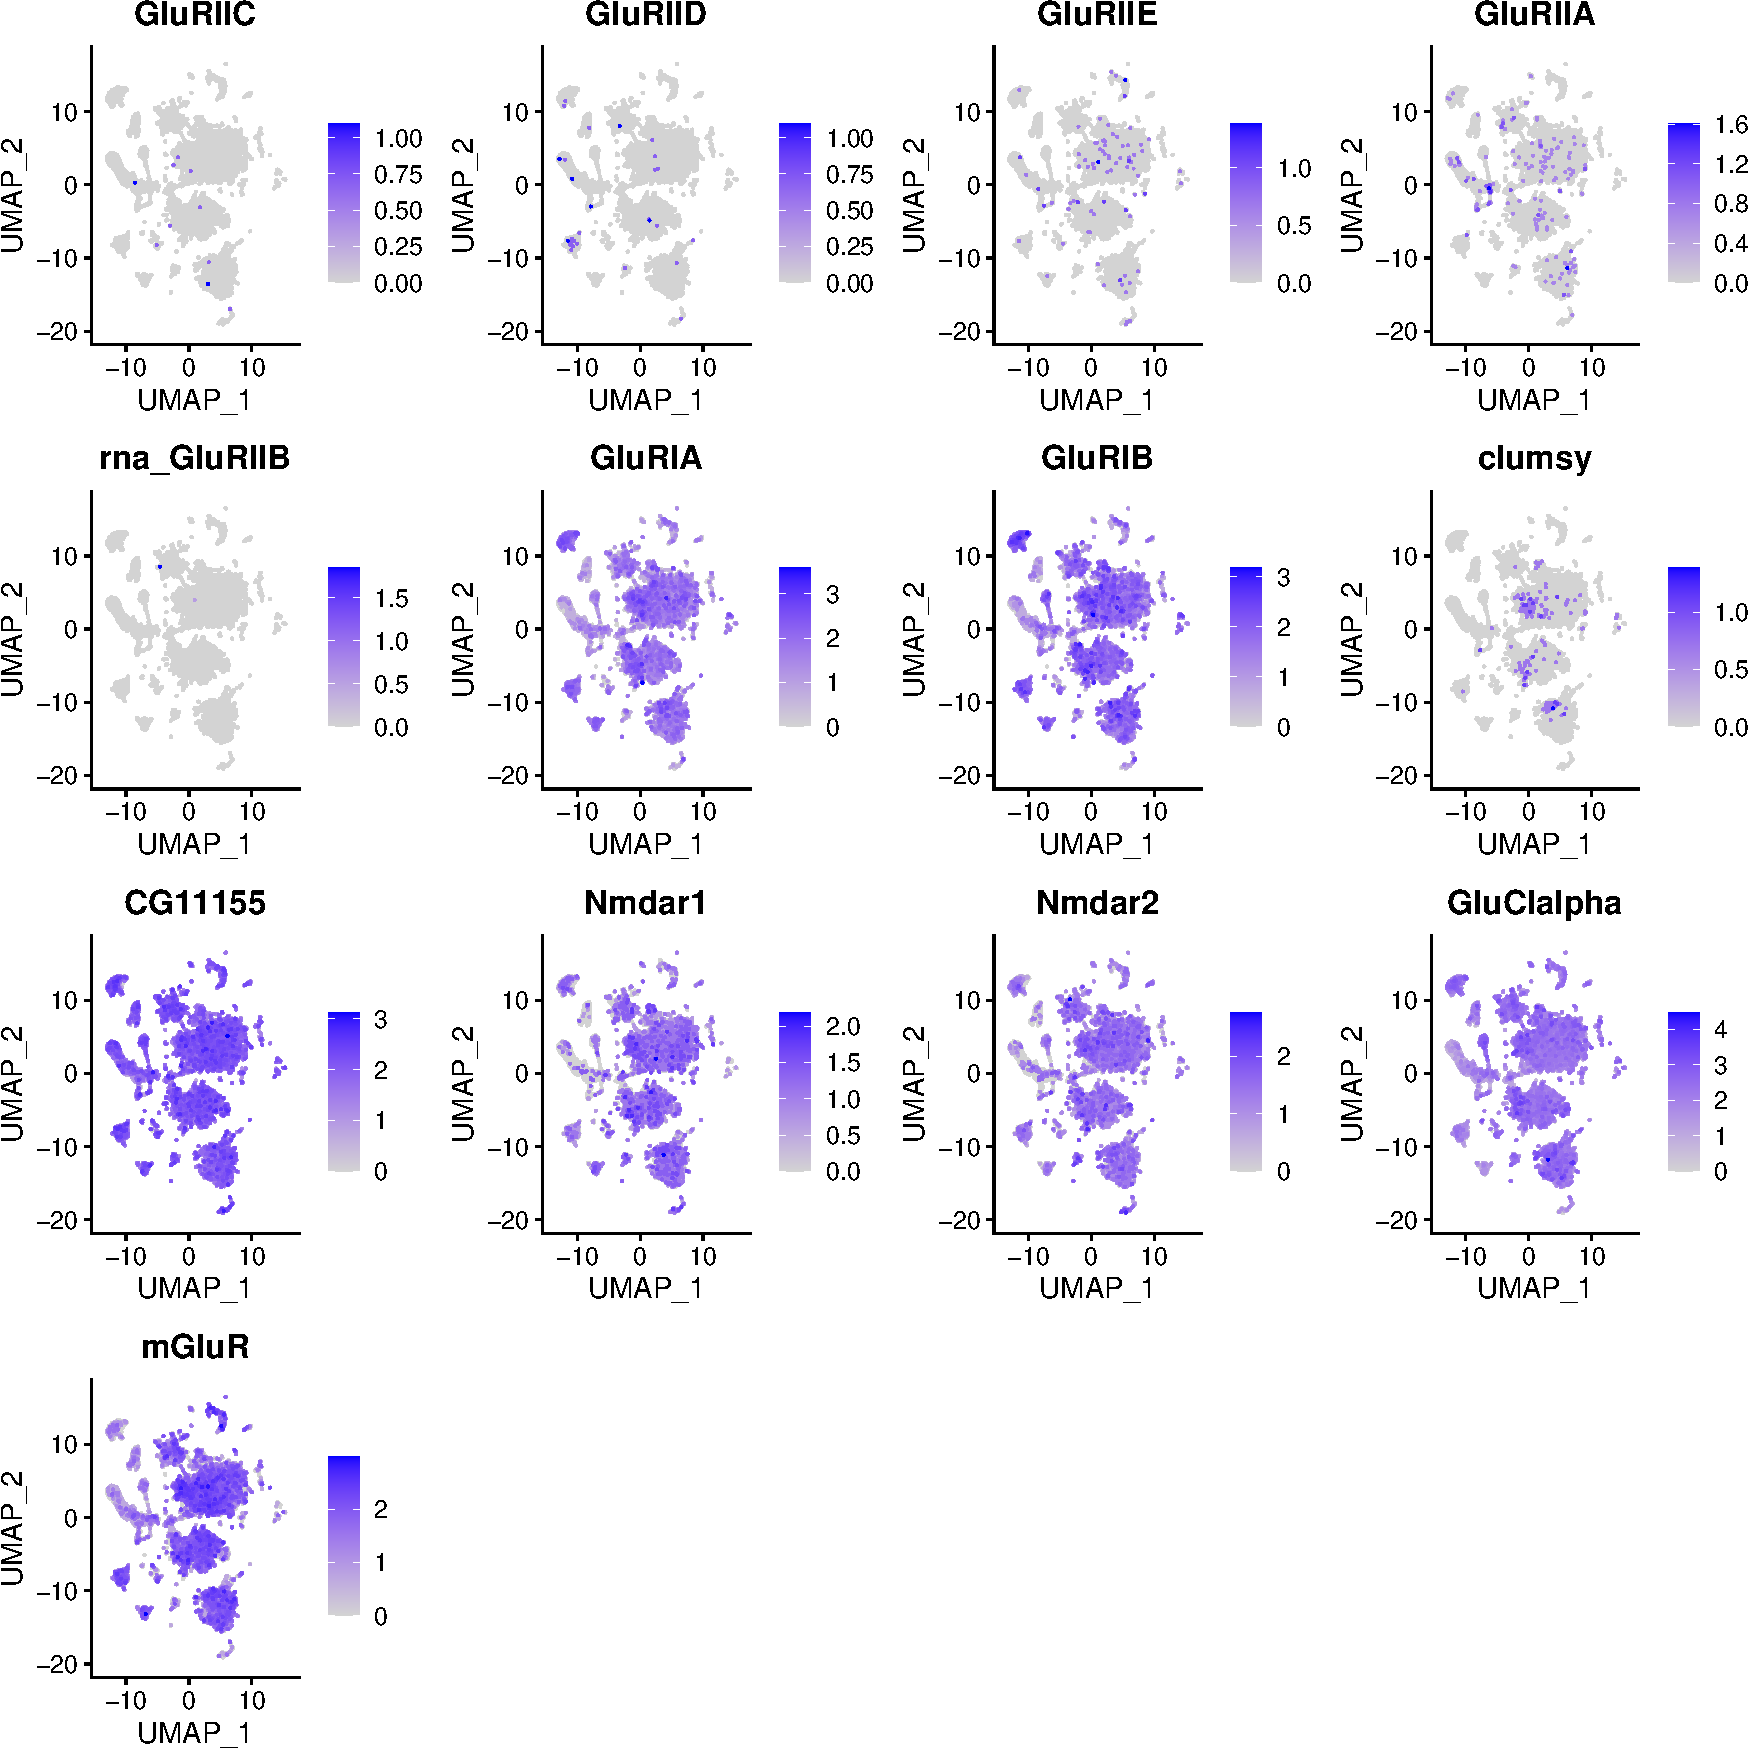
\includegraphics{~/projects/wilson-lab/nat-tech/images/GluR_scRNA/celltype_ann_glur_umap-1} \end{center}

\begin{center}\includegraphics{~/projects/wilson-lab/nat-tech/images/GluR_scRNA/celltype_ann_glur_dotplot_rna-1} \end{center}

\begin{center}\includegraphics{~/projects/wilson-lab/nat-tech/images/GluR_scRNA/celltype_ann_glur_dotplot_rna-2} \end{center}

\begin{center}\includegraphics{~/projects/wilson-lab/nat-tech/images/GluR_scRNA/celltype_ann_glur_dotplot_rna-3} \end{center}

\begin{center}\includegraphics{~/projects/wilson-lab/nat-tech/images/GluR_scRNA/celltype_ann_glur_dotplot_rna-4} \end{center}

\begin{center}\includegraphics{~/projects/wilson-lab/nat-tech/images/GluR_scRNA/celltype_ann_glur_dotplot_rna-5} \end{center}

\begin{center}\includegraphics{~/projects/wilson-lab/nat-tech/images/GluR_scRNA/celltype_ann_glur_dotplot_rna-6} \end{center}

\begin{center}\includegraphics{~/projects/wilson-lab/nat-tech/images/GluR_scRNA/celltype_ann_glur_dotplot_rna-7} \end{center}

\begin{center}\includegraphics{~/projects/wilson-lab/nat-tech/images/GluR_scRNA/celltype_ann_glur_dotplot_sct-1} \end{center}

\begin{center}\includegraphics{~/projects/wilson-lab/nat-tech/images/GluR_scRNA/celltype_ann_glur_dotplot_sct-2} \end{center}

\begin{center}\includegraphics{~/projects/wilson-lab/nat-tech/images/GluR_scRNA/celltype_ann_glur_dotplot_sct-3} \end{center}

\begin{center}\includegraphics{~/projects/wilson-lab/nat-tech/images/GluR_scRNA/celltype_ann_glur_dotplot_sct-4} \end{center}

\begin{center}\includegraphics{~/projects/wilson-lab/nat-tech/images/GluR_scRNA/celltype_ann_glur_dotplot_sct-5} \end{center}

\begin{center}\includegraphics{~/projects/wilson-lab/nat-tech/images/GluR_scRNA/celltype_ann_glur_dotplot_sct-6} \end{center}

\begin{center}\includegraphics{~/projects/wilson-lab/nat-tech/images/GluR_scRNA/celltype_ann_glur_dotplot_sct-7} \end{center}

\begin{center}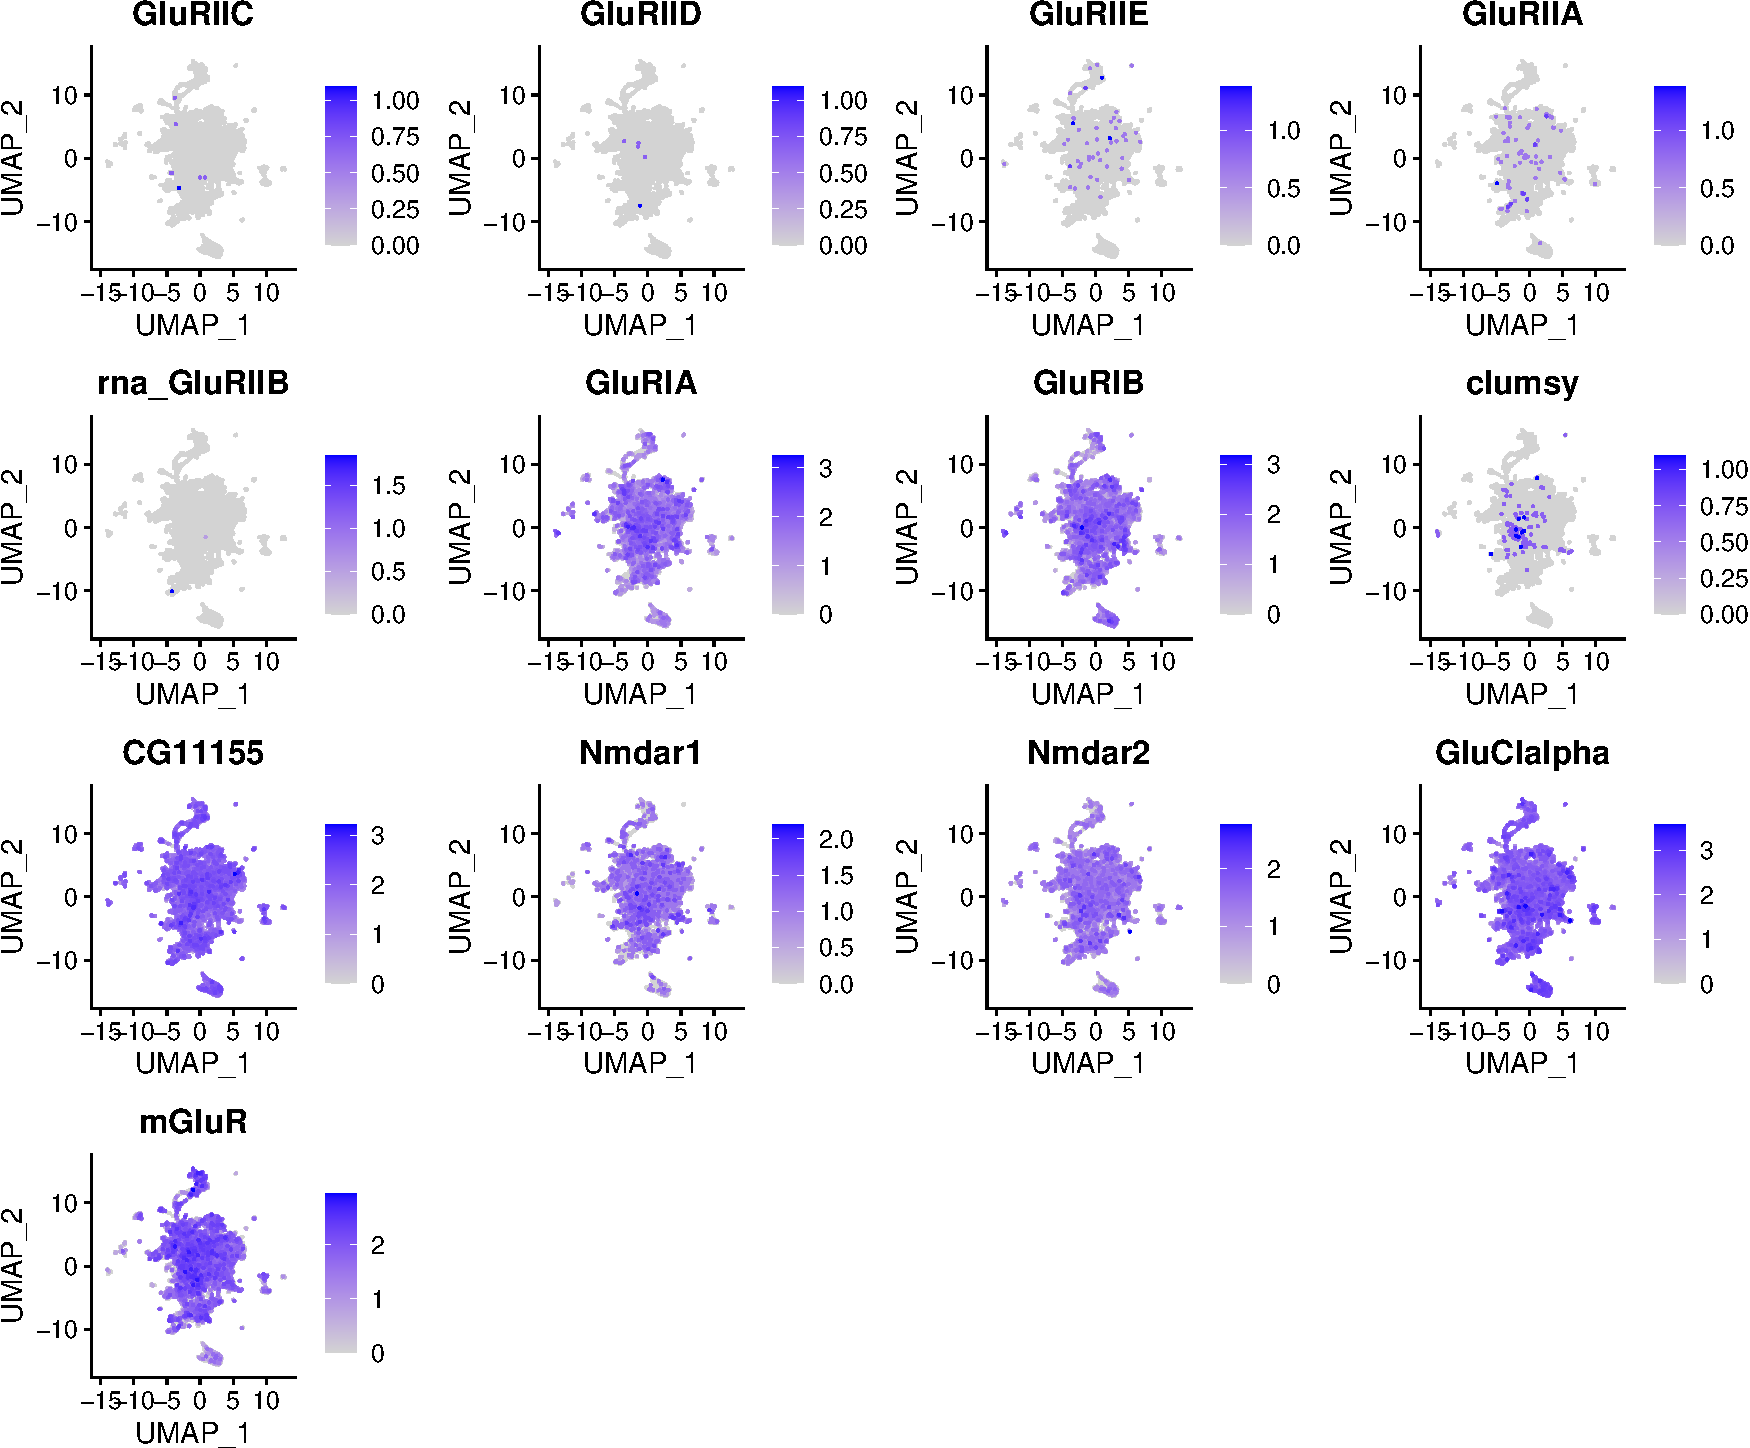
\includegraphics{~/projects/wilson-lab/nat-tech/images/GluR_scRNA/glur_feature_plots-1} \end{center}

\begin{center}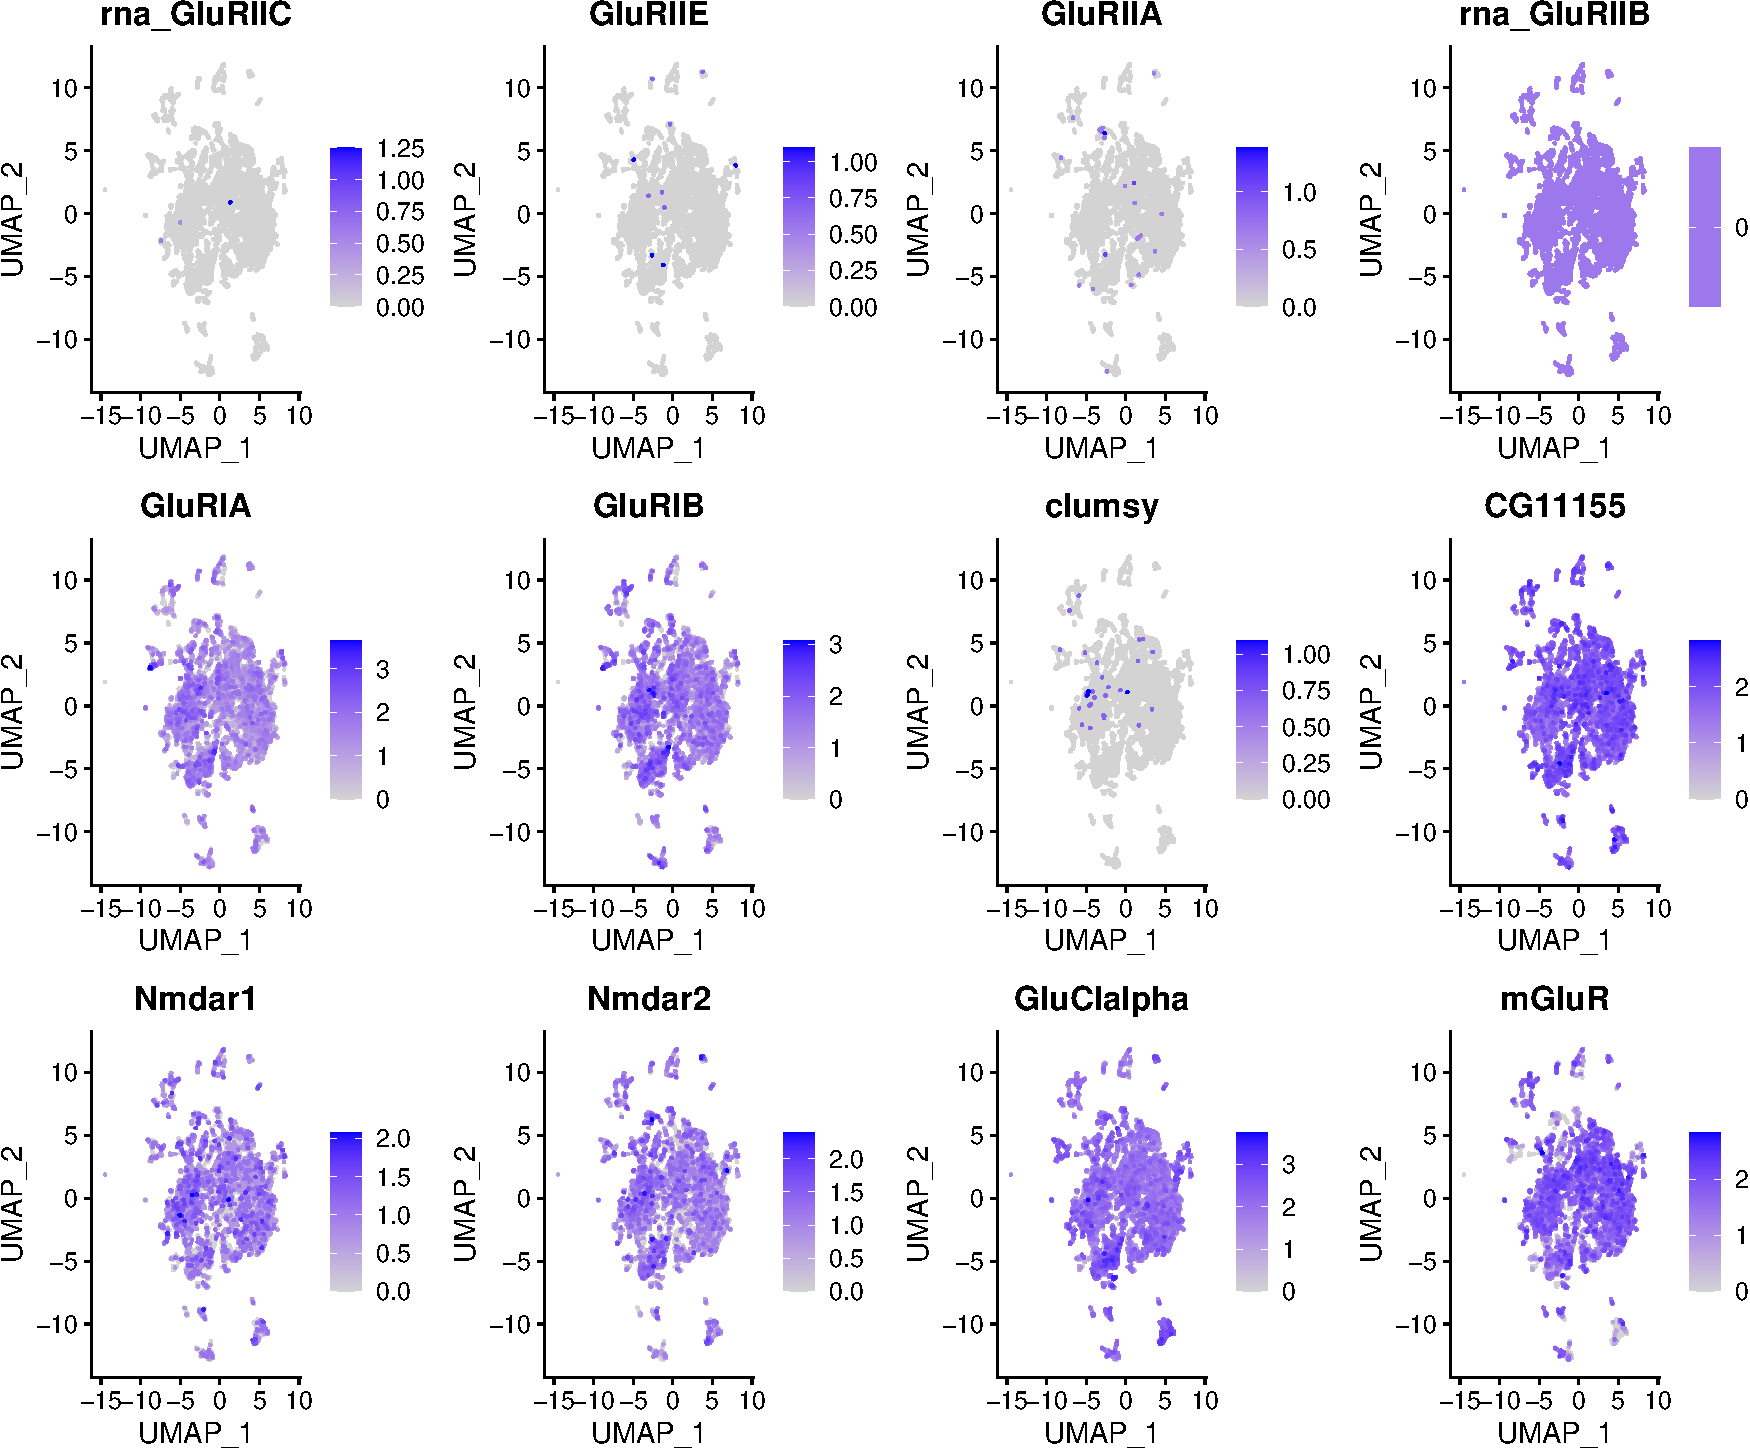
\includegraphics{~/projects/wilson-lab/nat-tech/images/GluR_scRNA/glur_feature_plots-2} \end{center}

\begin{center}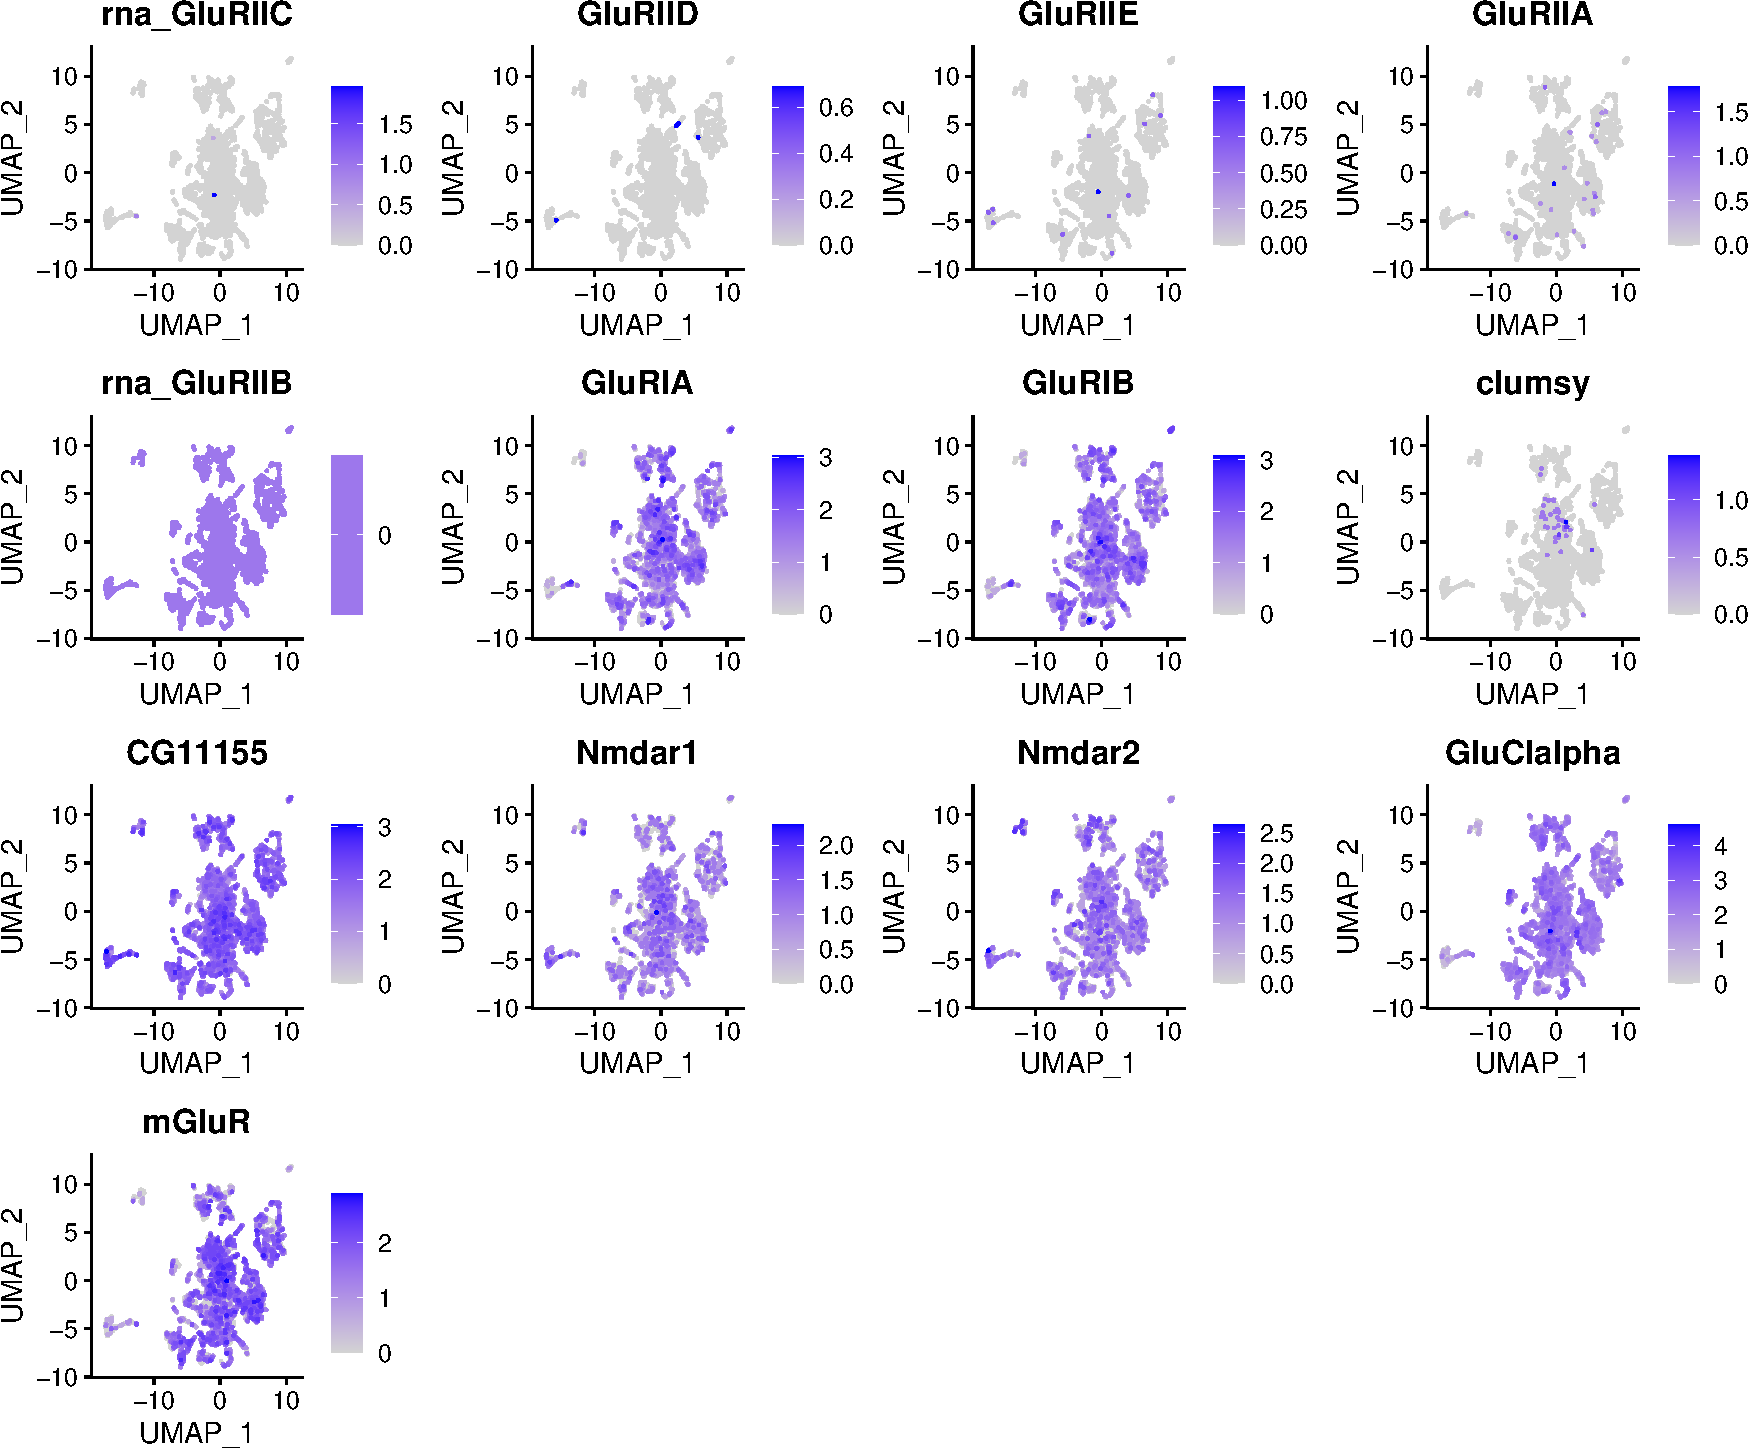
\includegraphics{~/projects/wilson-lab/nat-tech/images/GluR_scRNA/glur_feature_plots-3} \end{center}

\begin{center}\includegraphics{~/projects/wilson-lab/nat-tech/images/GluR_scRNA/glur_feature_plots-4} \end{center}

\begin{center}\includegraphics{~/projects/wilson-lab/nat-tech/images/GluR_scRNA/glur_feature_plots-5} \end{center}

\begin{center}\includegraphics{~/projects/wilson-lab/nat-tech/images/GluR_scRNA/glur_feature_plots-6} \end{center}

\begin{center}\includegraphics{~/projects/wilson-lab/nat-tech/images/GluR_scRNA/glur_feature_plots-7} \end{center}

How many neurons express more excitatory GluRs than inhibitory?

\begin{verbatim}
## [1] 0.8341747
\end{verbatim}

\begin{verbatim}
## [1] 0.868346
\end{verbatim}

\begin{verbatim}
## [1] 0.6214369
\end{verbatim}

\begin{verbatim}
## [1] 0.446133
\end{verbatim}

\begin{verbatim}
## [1] 0.8049145
\end{verbatim}

\begin{verbatim}
## [1] 0.4682499
\end{verbatim}

\hypertarget{speculative-central-complex}{%
\section{Speculative Central
Complex}\label{speculative-central-complex}}

Paper: \url{https://link.springer.com/article/10.1007/s00427-016-0542-7}
Several transcription factors remain detectable in a certain lineage
from the delaminating neuroblast to at least a subset of daughter cells
of that neuroblast like engrailed (Kumar et al.~2009), and Ct, Dan, Dll,
and Optix in type II neuroblasts (Bayraktar and Doe 2013).

\begin{center}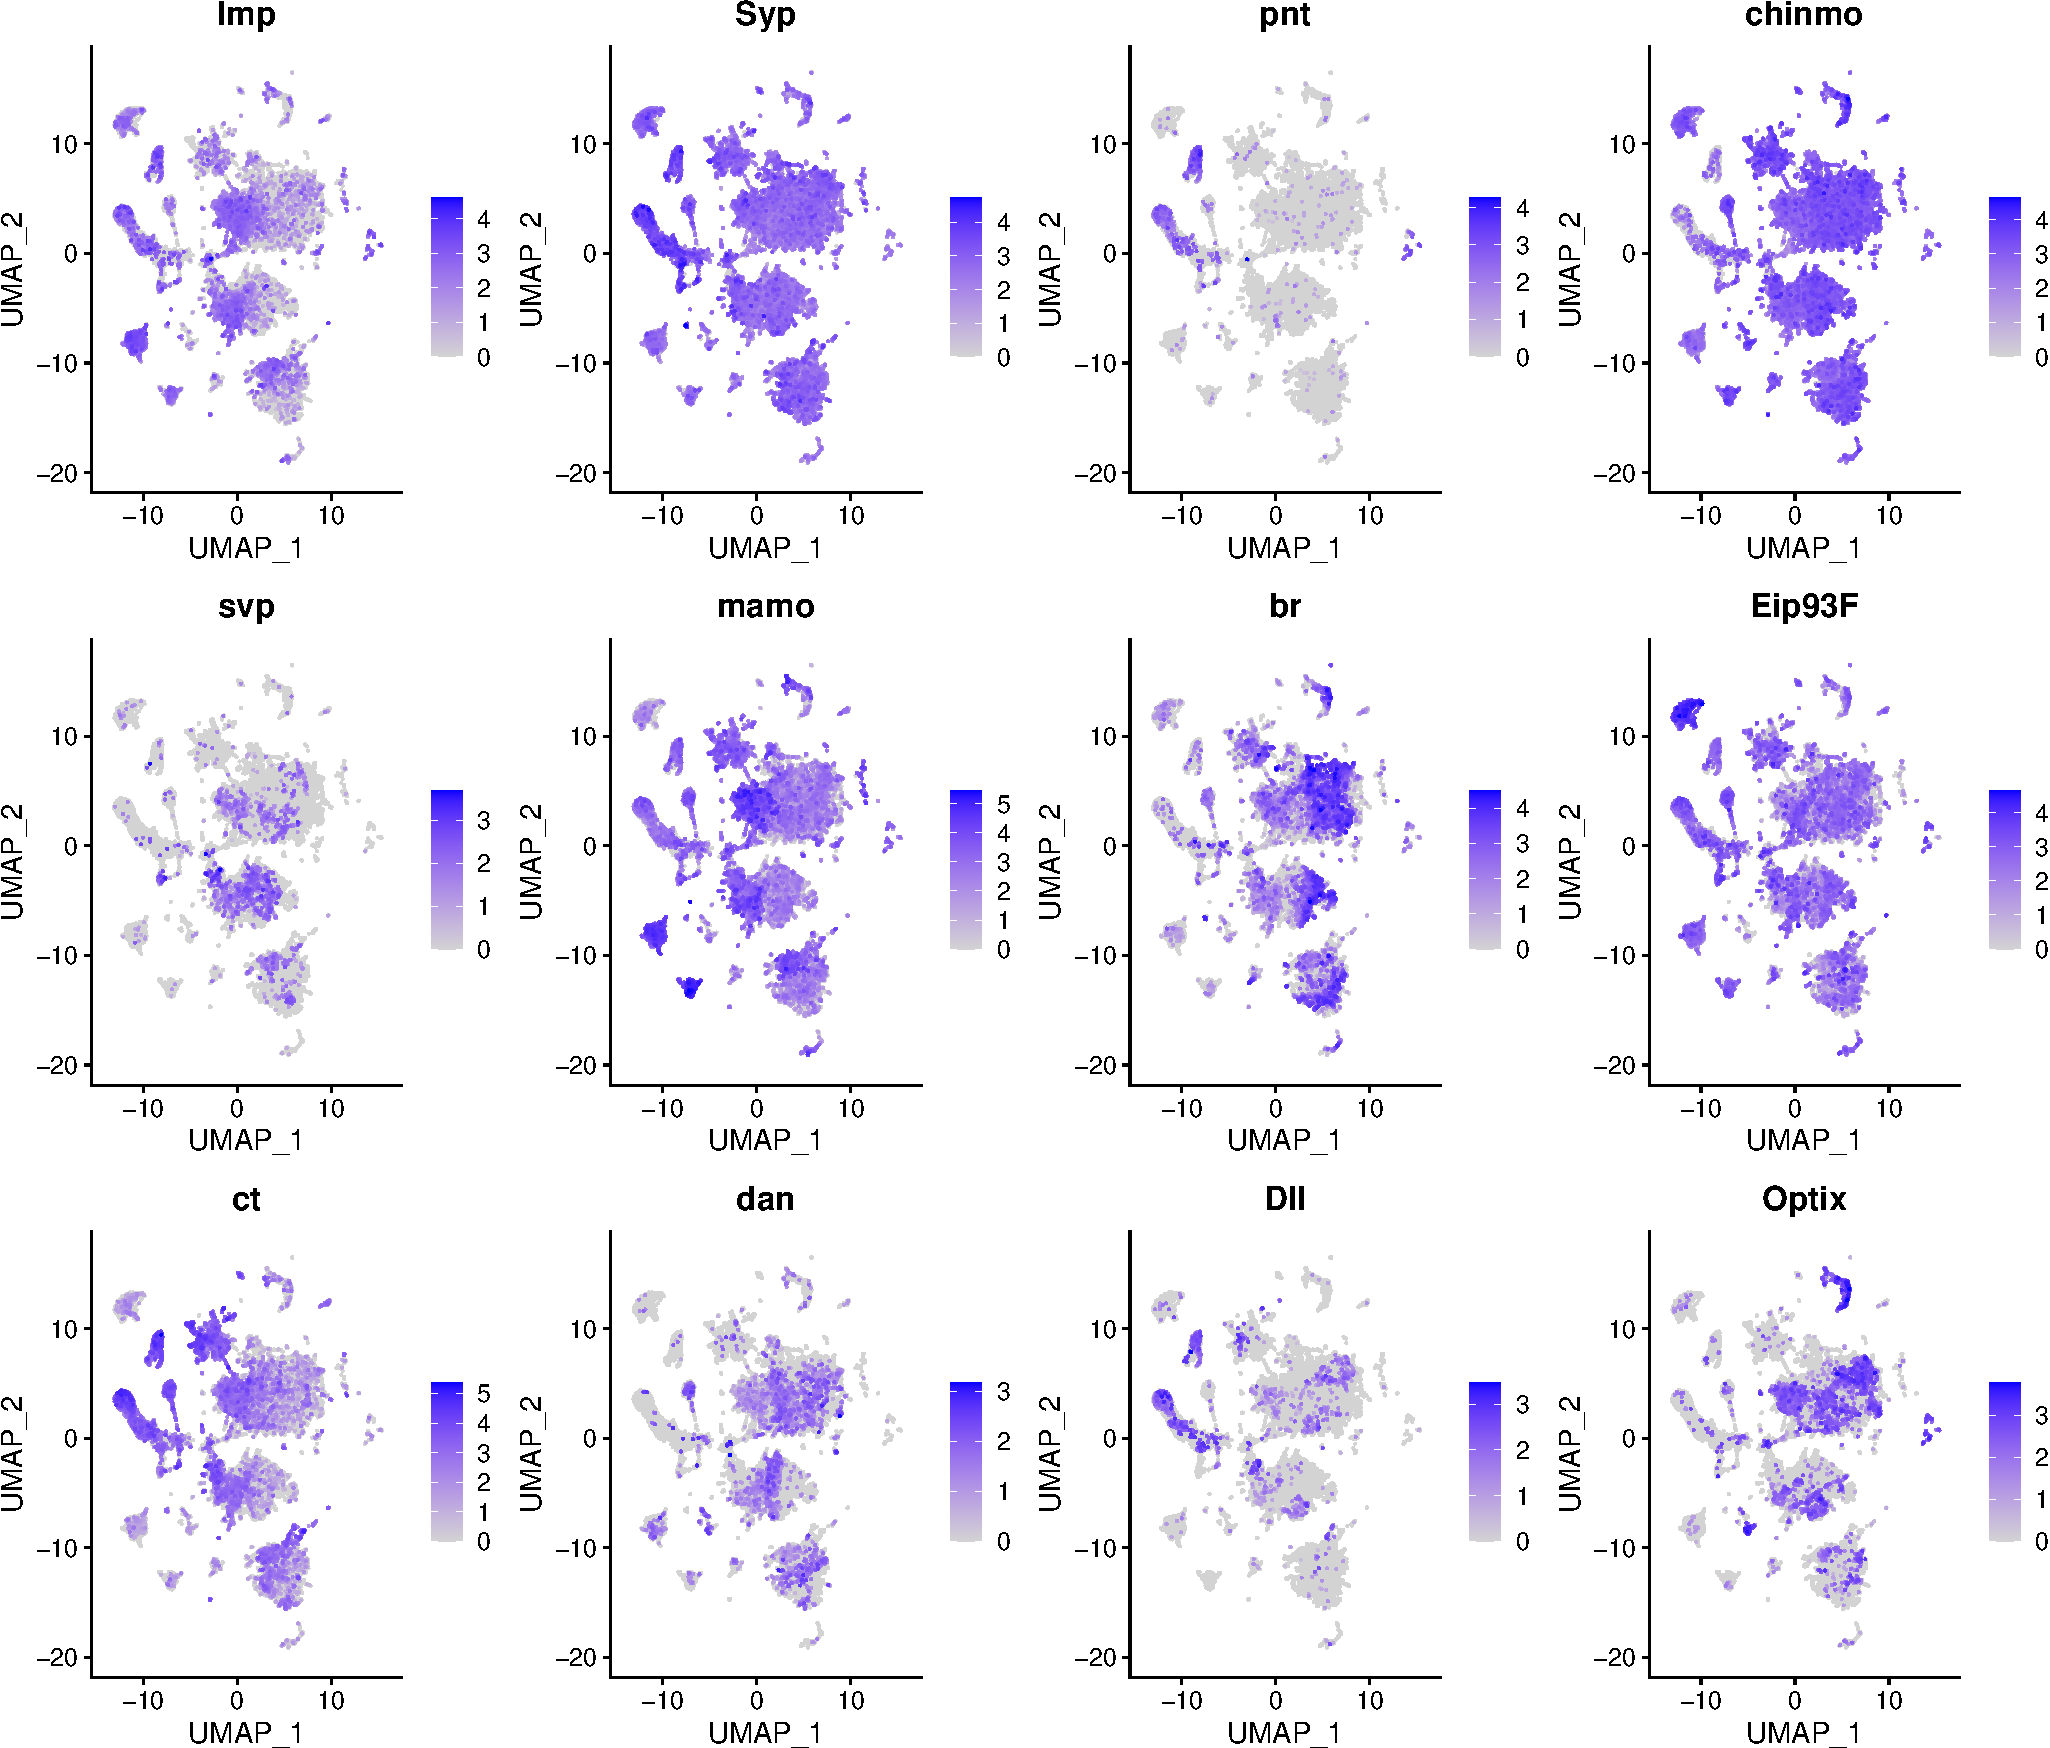
\includegraphics{~/projects/wilson-lab/nat-tech/images/GluR_scRNA/cx_markers_ump-1} \end{center}

\end{document}
